%\documentclass[a4,semhelv,landscape]{seminar}
\documentclass[landscape]{slides}
%\documentclass[landscape,aspectratio=169]{slides}
%\documentclass[pdf, default, slideBW, nocolorBG]{prosper}
\usepackage[left=0.2cm,top=0.2cm,right=0.2cm,bottom=0.2cm,nohead,nofoot]{geometry}
%\def\everyslide{\sffamily}
%\usepackage{fullpage}
\usepackage{graphicx}
\usepackage[usenames]{color}
%\usepackage{color}
\usepackage{verbatim}
\usepackage{nopageno}
\usepackage{setspace}
%\usepackage{times}
% define some nice colors
\definecolor{myred}{rgb}{0.6,0,0}
\definecolor{myblue}{rgb}{0,0.2,0.4}
\definecolor{mygreen}{rgb}{0,0.5,0.0}
\definecolor{mypurple}{cmyk}{0.5,1.0,0.0,0.0}
\definecolor{myorange}{cmyk}{0.0,0.75,1.0,0.0}
%\color{myblue}

\begin{document}
%%%%%%%%%%%%%%%%%%%%%%%%%%%%%%%%%%%%%%%%%%%%%%%%%%%%%%%%%%%%%%%%%%%%
%Slide 0 - title
\begin{slide}
\begin{center}
\large{\textbf{Validation and annotation of SARS-CoV-2 sequences \\ for GenBank using VADR}}

\normalsize

Eric Nawrocki \\
Staff Scientist \\

\medskip

\medskip

\medskip

\medskip

\medskip

\small
\begin{tabular}{c}
%Alejandro Sch\"{a}ffer's group \\
%\\
Computational Biology Branch \\
%National Center for Biotechnology Information\\
National Center for Biotechnology Information\\
%National Institutes of Health\\
National Library of Medicine \\
\\
\end{tabular}

\vspace{0.1in}


\includegraphics[width=2.5in]{figs/NIH_NLM_ABRV_2C_4-white}

\includegraphics[width=2.5in]{figs/ncbi-logo}

\end{center}
\end{slide}
%%%%%%%%%%%%%%%%%%%%%%%%%%%%%%%%%%%%%%%%%%%%%%%%%%%%%%%%%%%%%%%%%%%%%%
\begin{slide}
\begin{center}
\large{\textbf{GenBank indexers handle incoming sequence submissions}}
\end{center}

\center{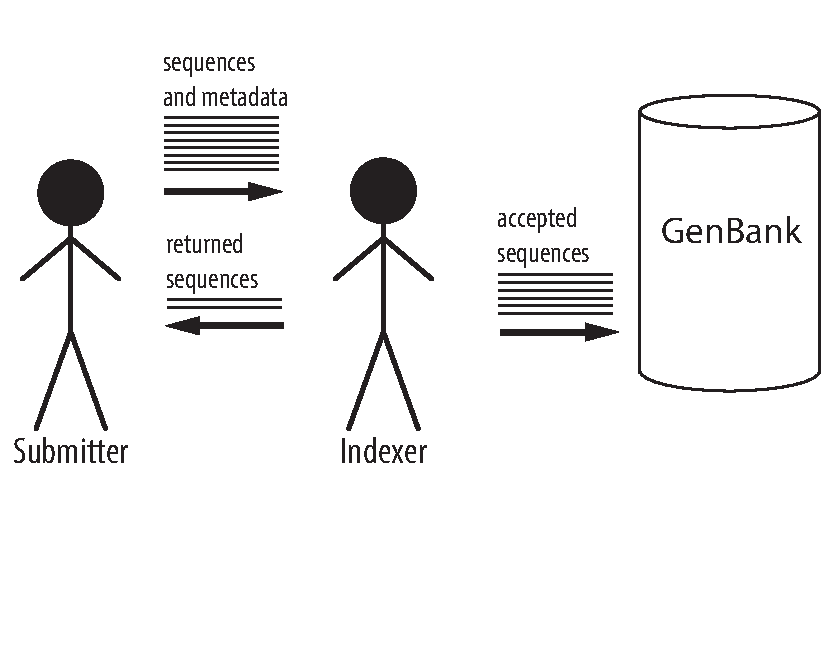
\includegraphics[width=9in]{figs/spheres-submission-schematic-1}}

\vfill
\end{slide}
%%%%%%%%%%%%%%%%%%%%%%%%%%%%%%%%%%%%%%%%%%%%%%%%%%%%%%%%%%%%%%%%%%%%%%
\begin{slide}
\begin{center}

\includegraphics[width=10in]{figs/vadr-title-paper}

\begin{itemize}
\item general tool for reference-based annotation of viral sequences
\item used for dengue virus and norovirus submissions since 2018
\item used for SARS-CoV-2 submissions since March 2020 
\end{itemize}

\vfill
\end{center}
\end{slide}
%%%%%%%%%%%%%%%%%%%%%%%%%%%%%%%%%%%%%%%%%%%%%%%%%%%%%%%%%%%%%%%%%%%%%%
\begin{slide}
\begin{center}
\large{\textbf{VADR assists GenBank indexers: \\ Each sequence \textcolor{green}{PASSes} or \textcolor{red}{FAILs}}}
\end{center}

\center{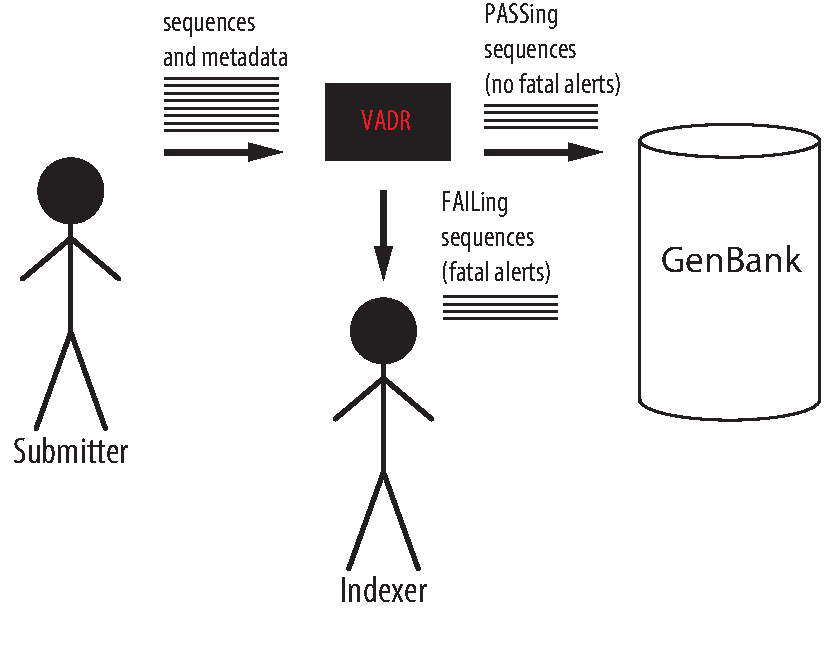
\includegraphics[width=9in]{figs/spheres-submission-schematic-2}}

\vfill
\end{slide}
%%%%%%%%%%%%%%%%%%%%%%%%%%%%%%%%%%%%%%%%%%%%%%%%%%%%%%%%%%%%%%%%%%%%%%
\begin{slide}
\begin{center}
\textbf{Indexers decide fate of most \textcolor{red}{FAILing} sequences\\ but some are sent directly back to submitter with error reports}
\end{center}

%\center{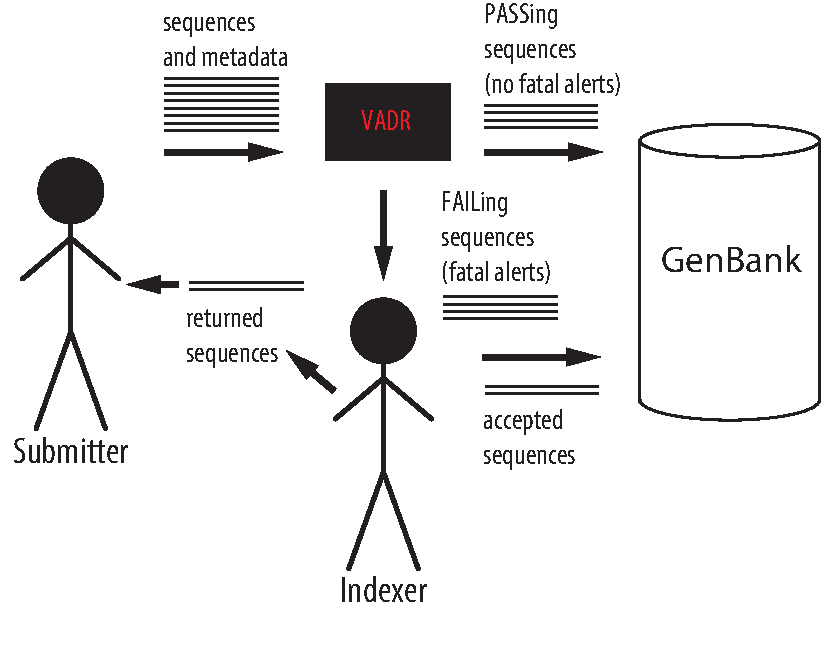
\includegraphics[width=9in]{figs/spheres-submission-schematic-3}}
\center{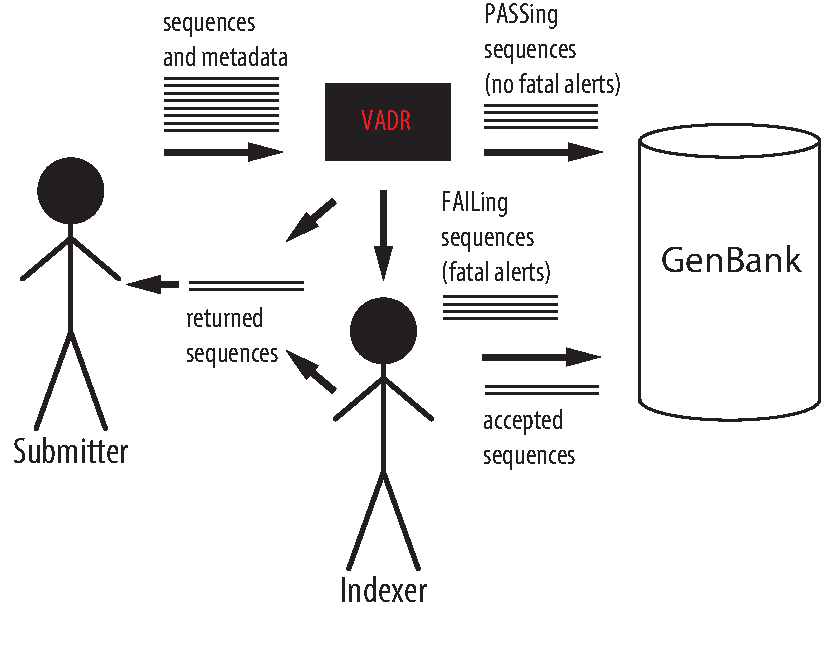
\includegraphics[width=9in]{figs/spheres-submission-schematic-4}}

\vfill
\end{slide}
%%%%%%%%%%%%%%%%%%%%%%%%%%%%%%%%%%%%%%%%%%%%%%%%%%%%%%%%%%%%%%%%%%%%%%
\begin{slide}
\begin{center}
\large{\textbf{VADR builds a reference model of a \\ RefSeq and its features}}
\end{center}

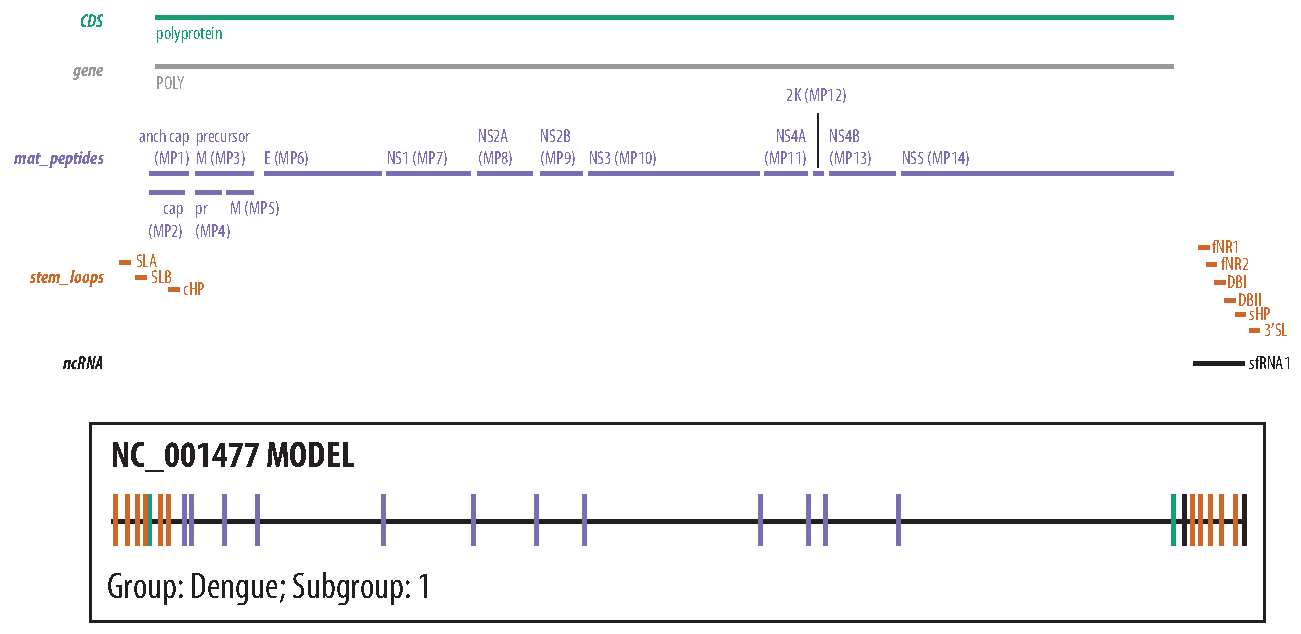
\includegraphics[width=10.5in]{figs/dengue-features}

\vfill
\end{slide}
%%%%%%%%%%%%%%%%%%%%%%%%%%%%%%%%%%%%%%%%%%%%%%%%%%%%%%%%%%%%%%%%%%%%%%
\begin{slide}
\begin{center}
%\textbf{\texttt{v-annotate.pl} annotates each sequence using its
\large{\textbf{VADR validates and annotates each input sequence \\ using its 
  best-matching model}}

\begin{itemize}
\item Each sequence $S$ proceeds through 4 stages:
%\item For each sequence $S$:
\small
\begin{enumerate}
%\item \textbf{Classification}: compare $S$ to all models to find best matching model $M$
\item \textbf{Classification}
%\item \textbf{Coverage determination}: search $M$ against $S$ to find 'hits'
\item \textbf{Coverage determination}
%\item \textbf{Alignment}: align $S$ to $M$ and map features from $M$ to $S$
\item \textbf{Alignment}
%\item \textbf{Protein validation}: compare predicted CDS in $S$ to proteins
\item \textbf{Protein validation}
\end{enumerate}
\end{itemize}

\normalsize
\emph{Different types of alerts are identified and reported at each stage}

\end{center}

\vfill
\end{slide}
%%%%%%%%%%%%%%%%%%%%%%%%%%%%%%%%%%%%%%%%%%%%%%%%%%%%%%%%%%%%%%%%%%%%%%
\begin{slide}
\begin{center}

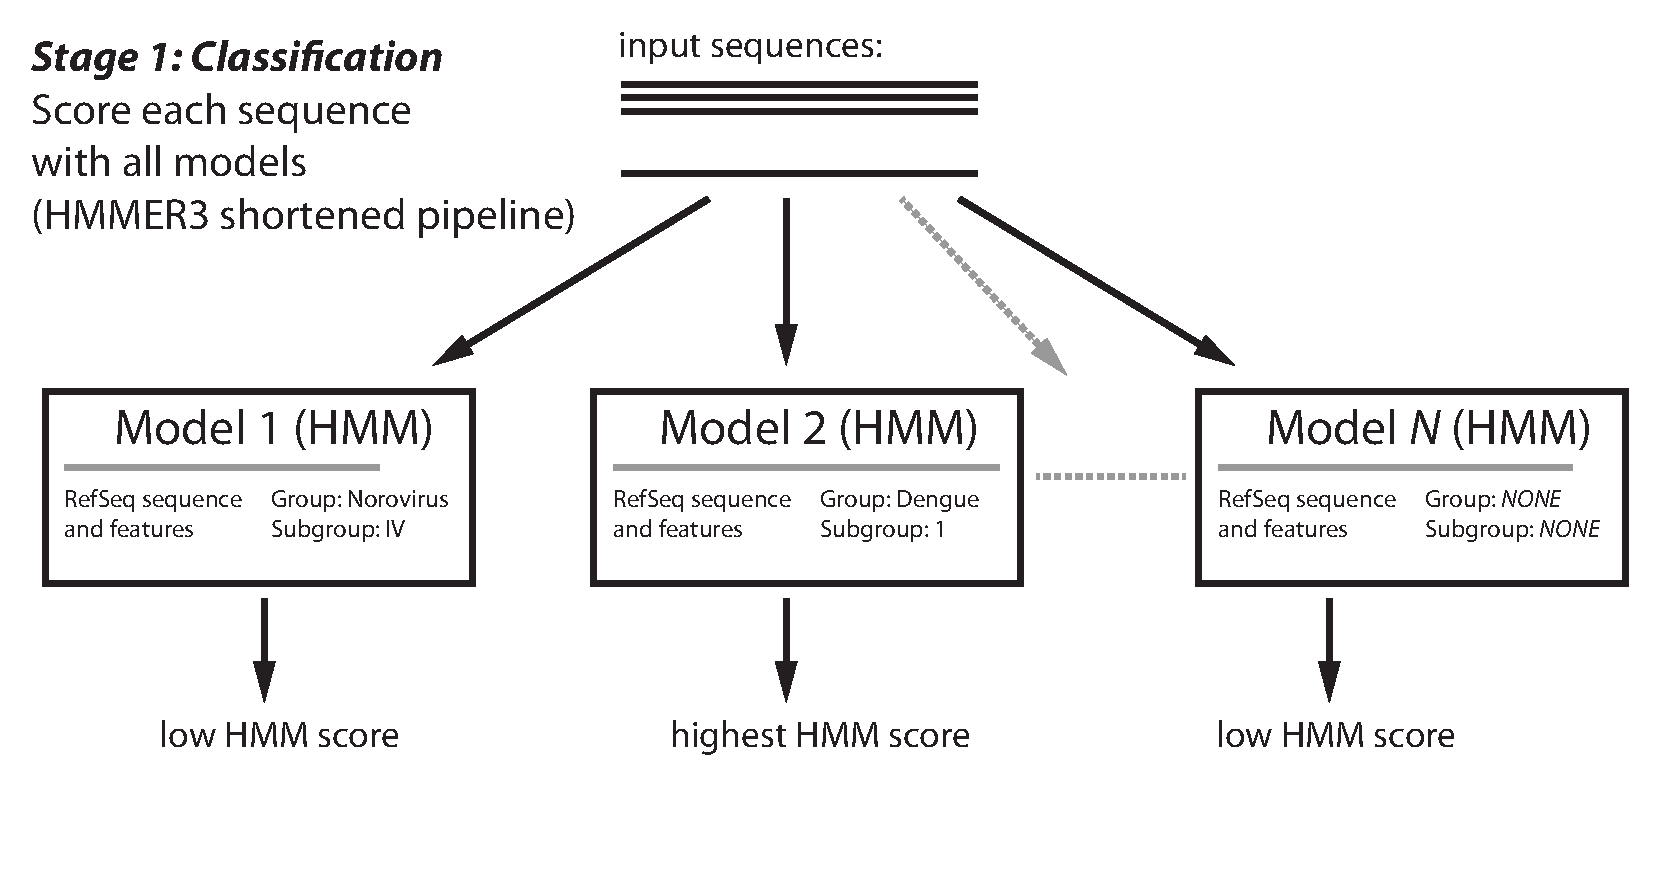
\includegraphics[width=9.5in]{figs/v-annotate-stage1-1}

\end{center}
\vfill
\end{slide}
%%%%%%%%%%%%%%%%%%%%%%%%%%%%%%%%%%%%%%%%%%%%%%%%%%%%%%%%%%%%%%%%%%%%%%
\begin{slide}
\begin{center}

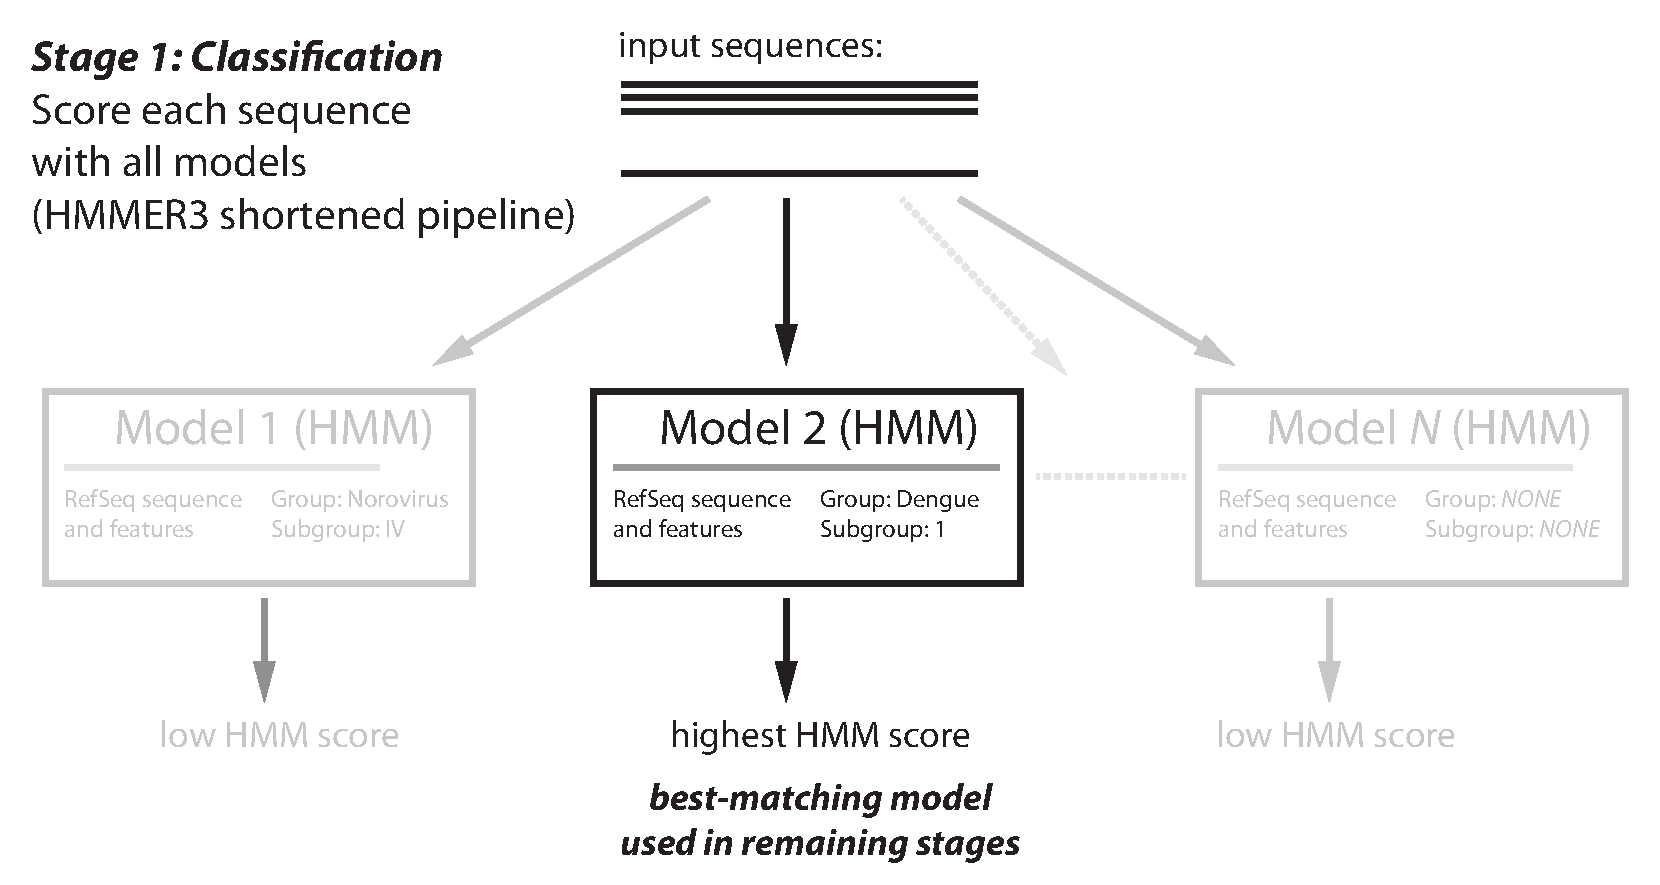
\includegraphics[width=9.5in]{figs/v-annotate-stage1-2}

\end{center}
\vfill
\end{slide}
%%%%%%%%%%%%%%%%%%%%%%%%%%%%%%%%%%%%%%%%%%%%%%%%%%%%%%%%%%%%%%%%%%%%%%
\begin{slide}
\begin{center}

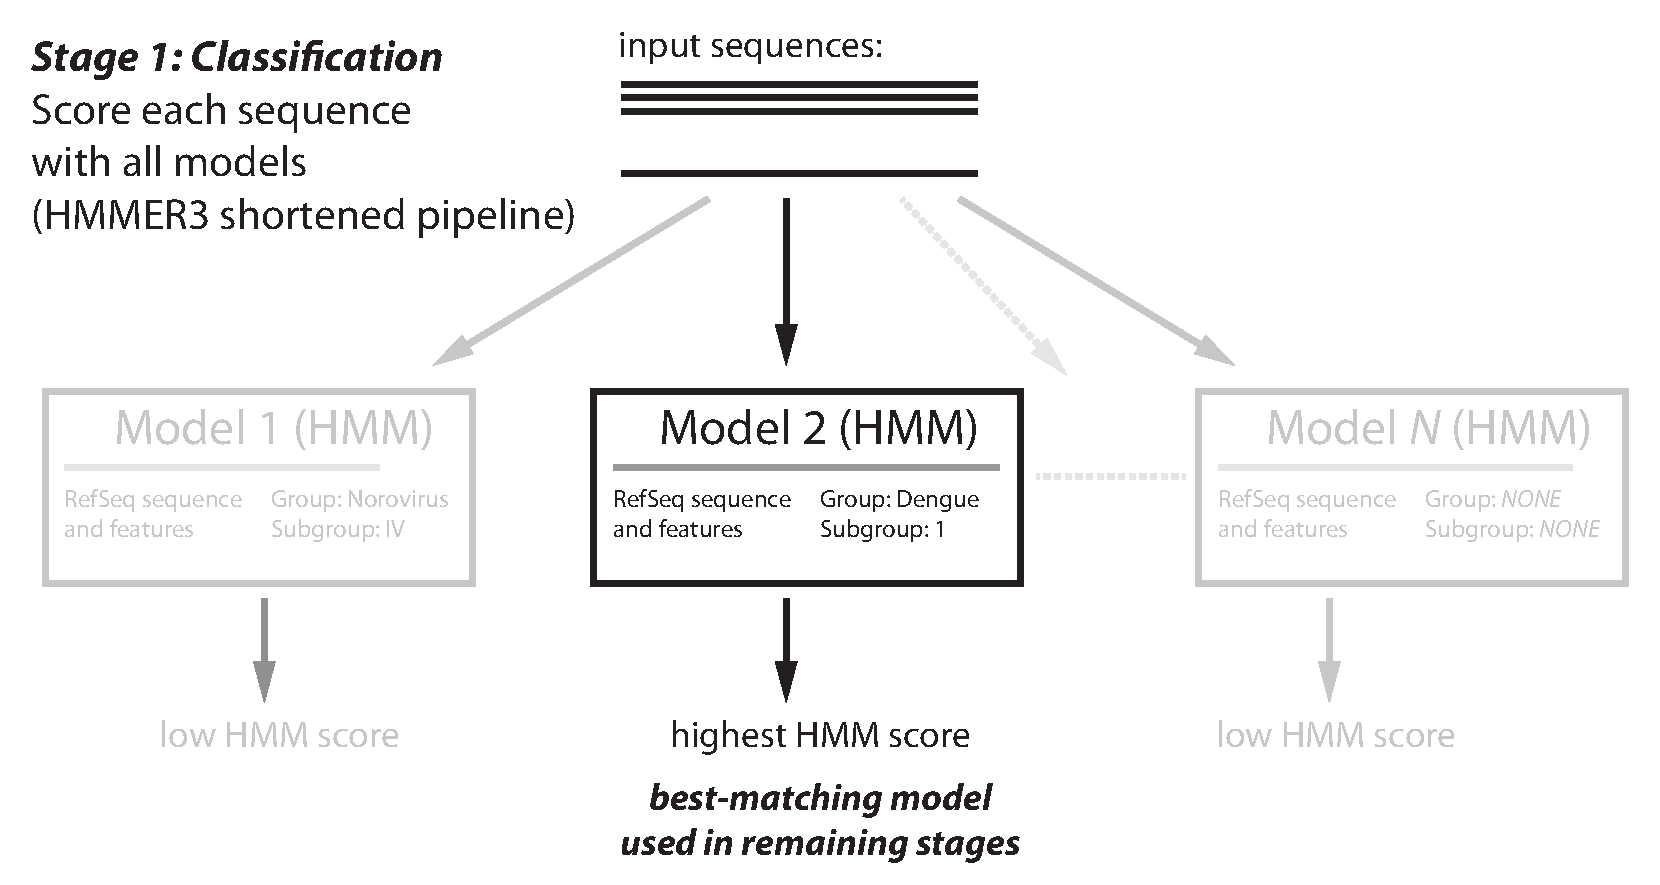
\includegraphics[width=9.5in]{figs/v-annotate-stage1-2}

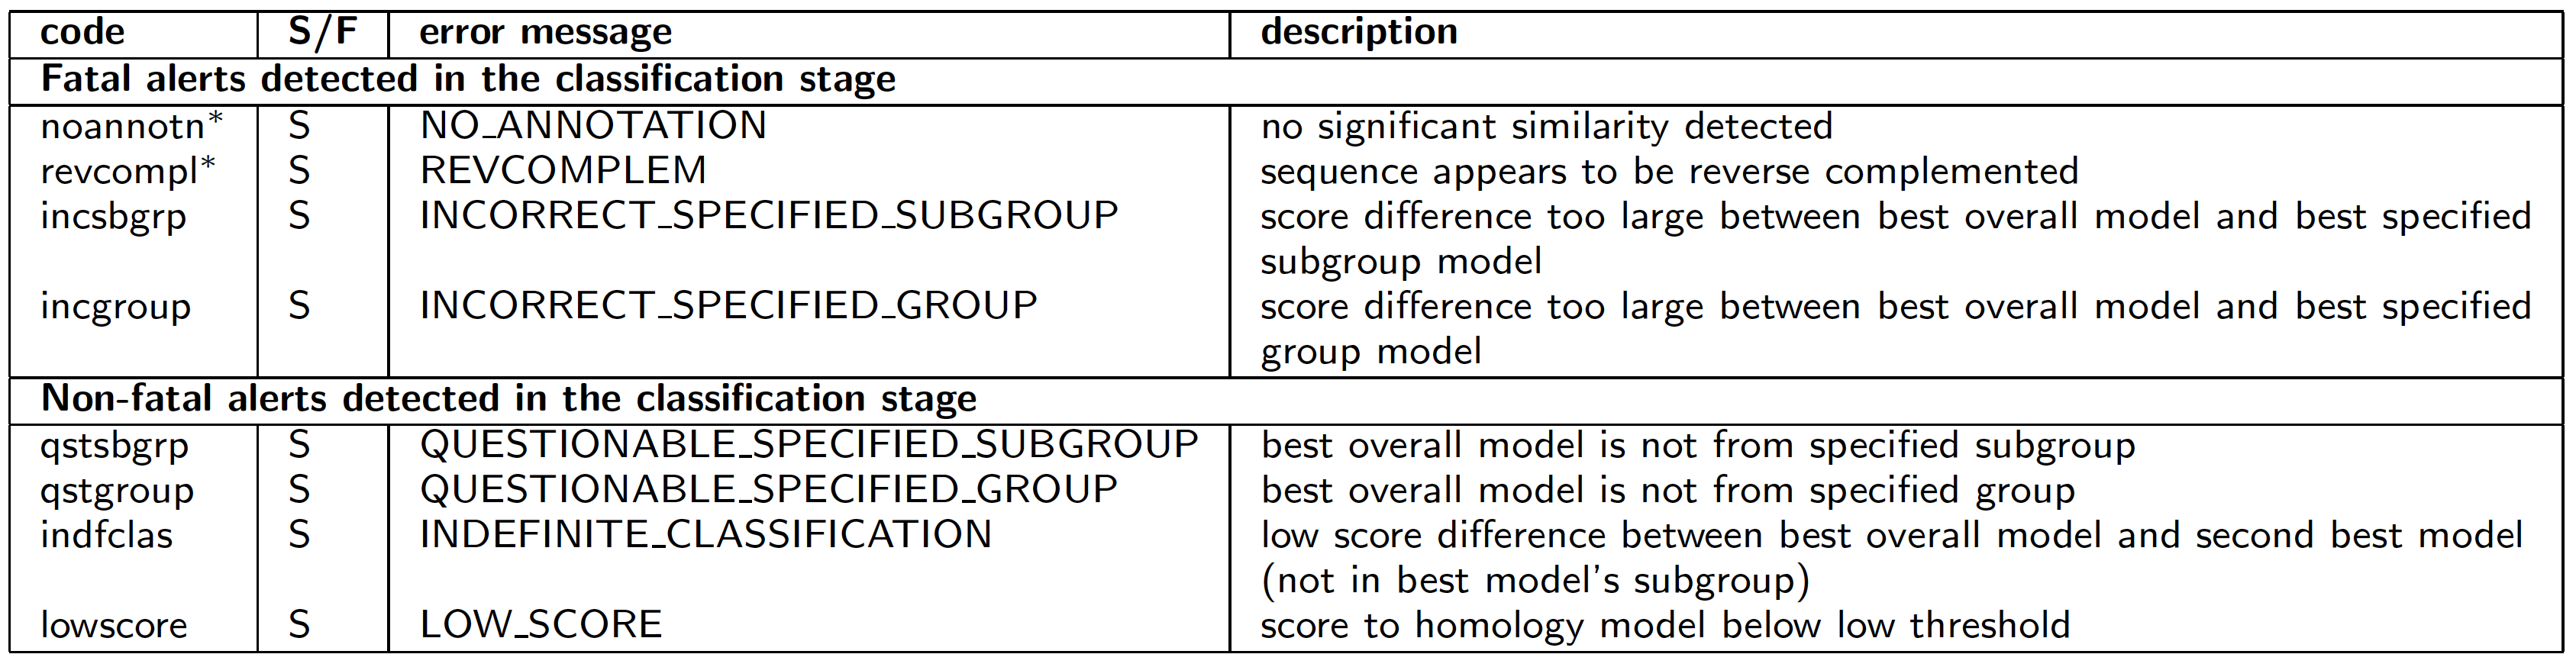
\includegraphics[width=10.5in]{figs/ss-class-alert-list}

\end{center}
\vfill
\end{slide}
%%%%%%%%%%%%%%%%%%%%%%%%%%%%%%%%%%%%%%%%%%%%%%%%%%%%%%%%%%%%%%%%%%%%%%
\begin{slide}
\begin{center}

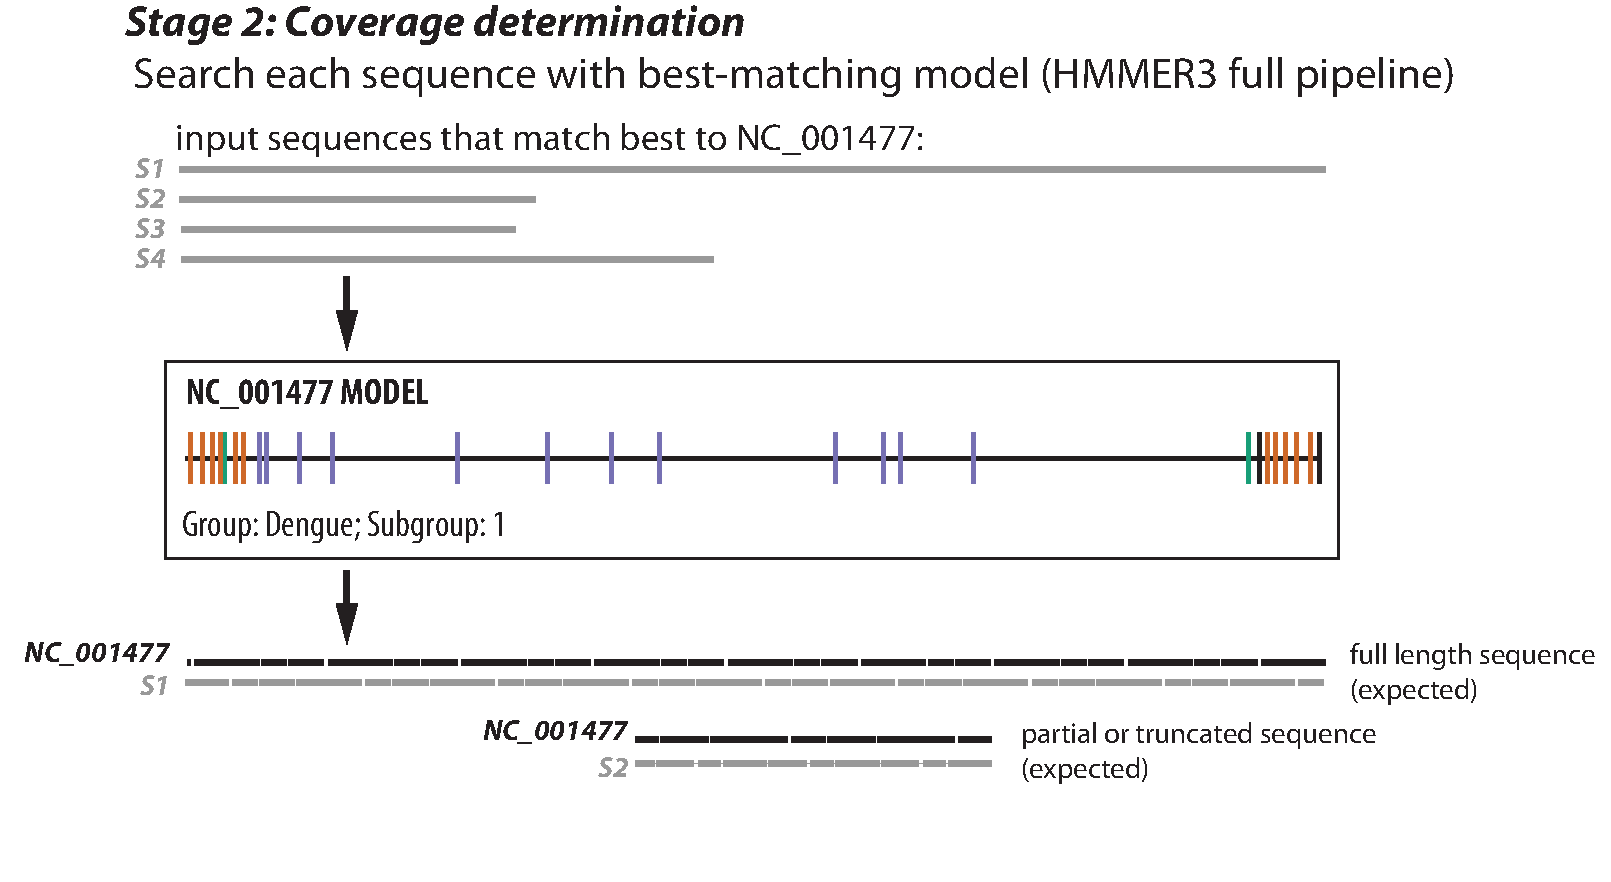
\includegraphics[width=10.5in]{figs/v-annotate-stage2-1}

\end{center}
\vfill
\end{slide}
%%%%%%%%%%%%%%%%%%%%%%%%%%%%%%%%%%%%%%%%%%%%%%%%%%%%%%%%%%%%%%%%%%%%%%
\begin{slide}
\begin{center}

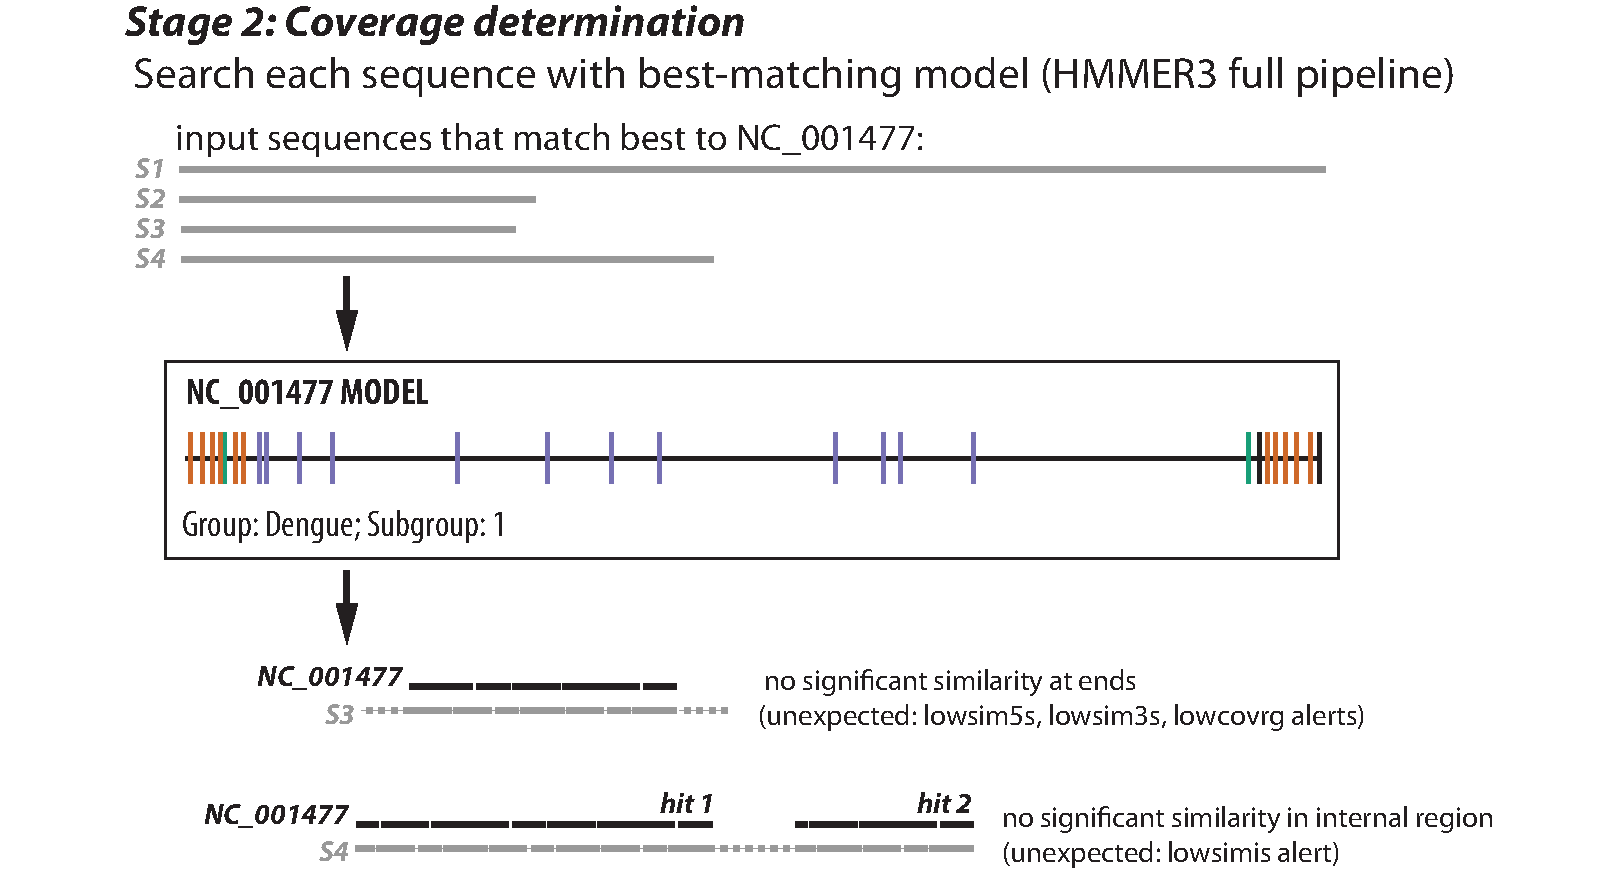
\includegraphics[width=10.5in]{figs/v-annotate-stage2-2}
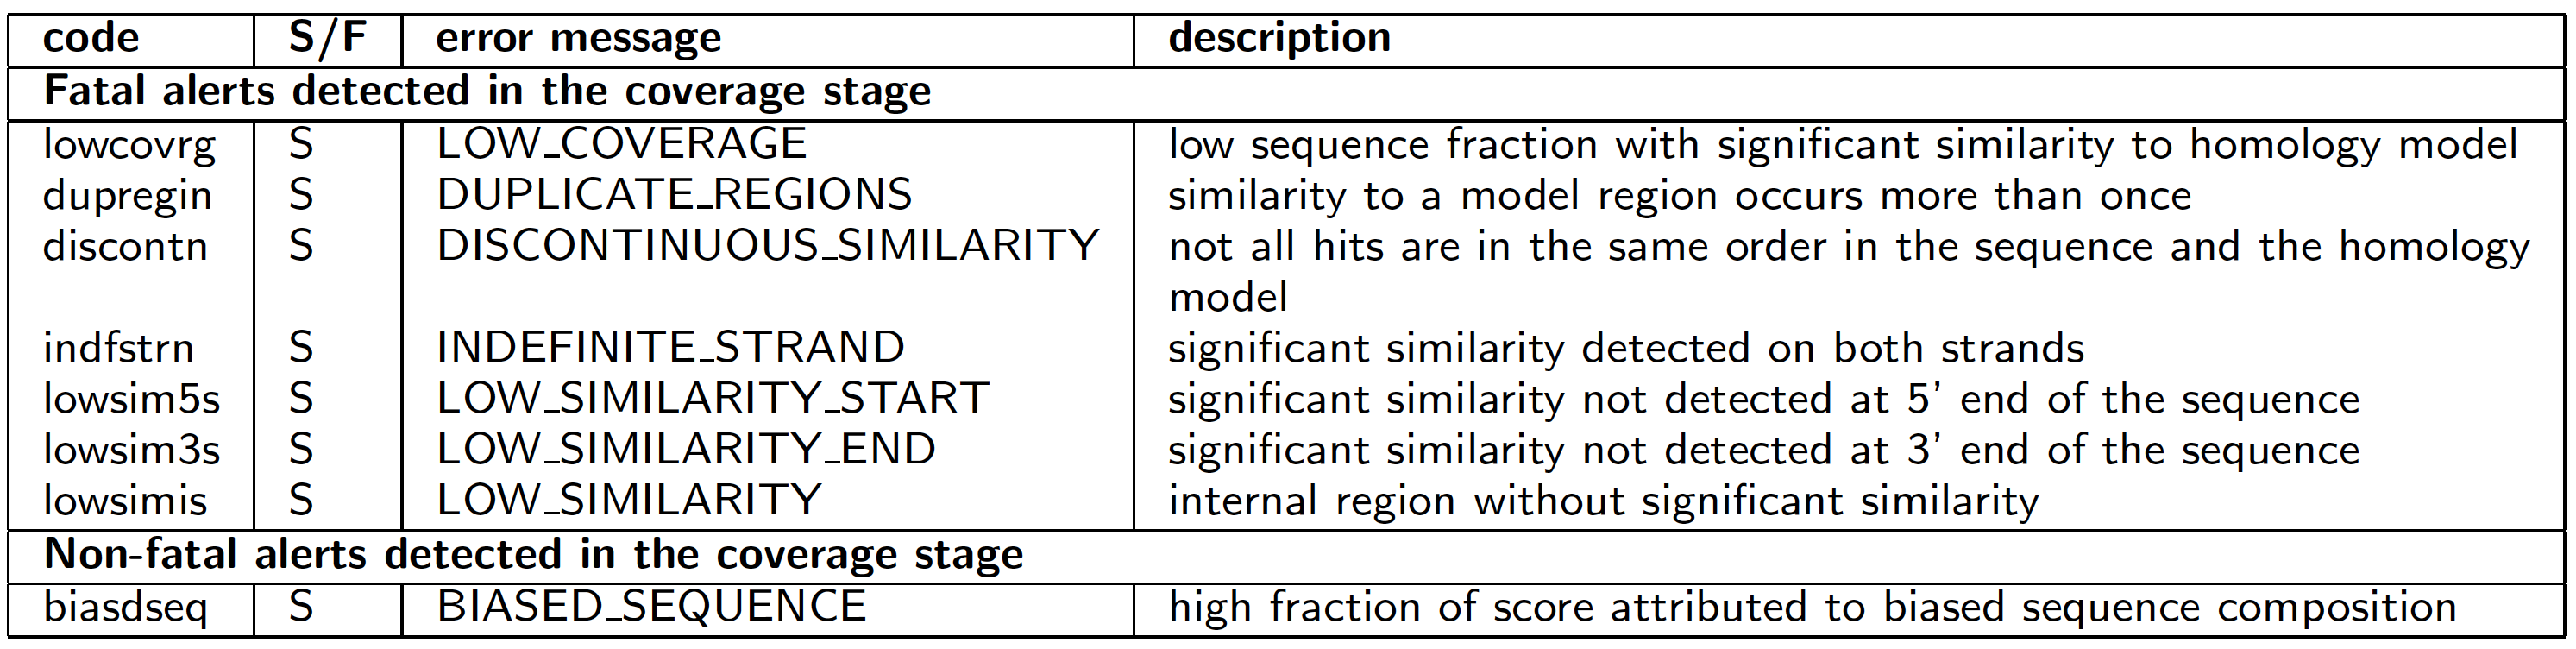
\includegraphics[width=10in]{figs/ss-coverage-alert-list}
\end{center}

\vfill
\end{slide}
%%%%%%%%%%%%%%%%%%%%%%%%%%%%%%%%%%%%%%%%%%%%%%%%%%%%%%%%%%%%%%%%%%%%%%
\begin{slide}
\begin{center}

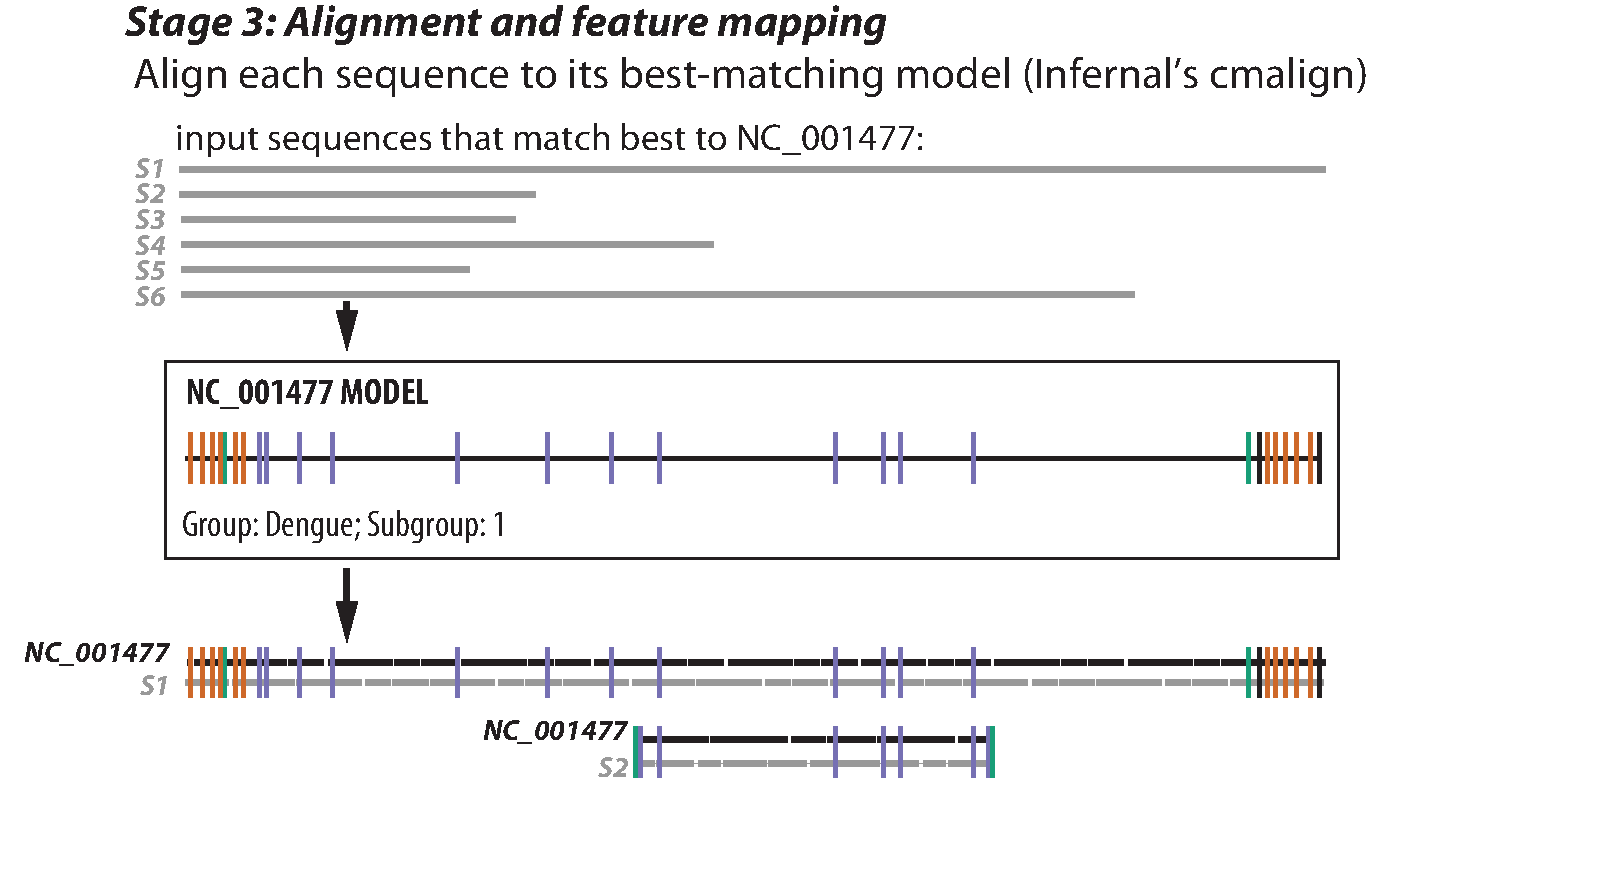
\includegraphics[width=10.5in]{figs/v-annotate-stage3-1}
\end{center}

\vfill
\end{slide}
%%%%%%%%%%%%%%%%%%%%%%%%%%%%%%%%%%%%%%%%%%%%%%%%%%%%%%%%%%%%%%%%%%%%%%
%\begin{slide}
%\begin{center}
%
%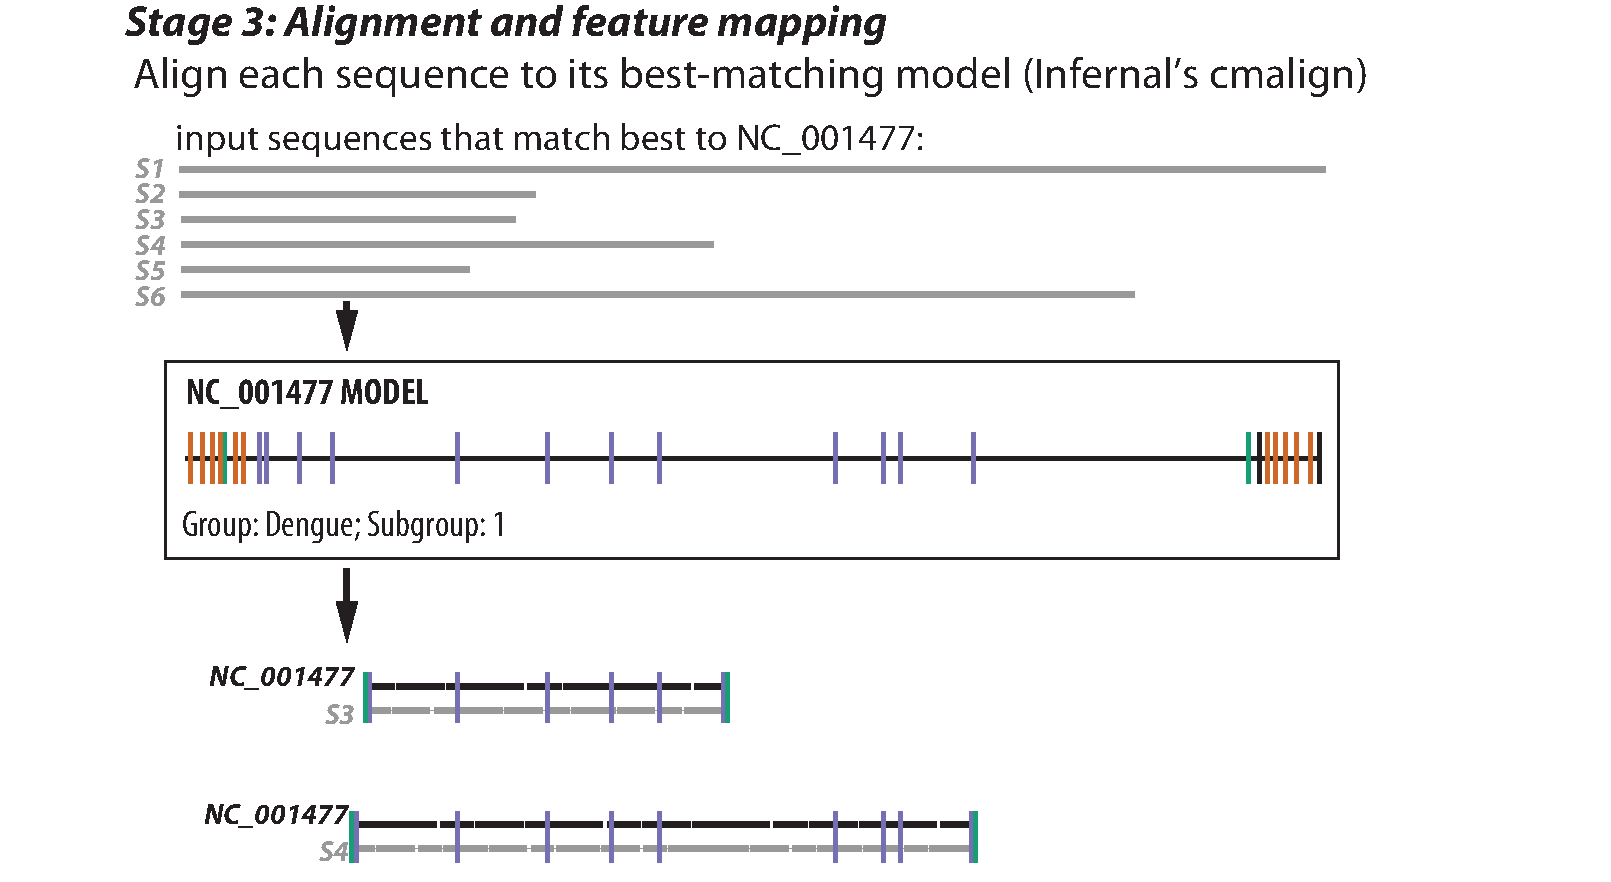
\includegraphics[width=10.5in]{figs/v-annotate-stage3-2}
%\end{center}
%
%\vfill
%\end{slide}
%%%%%%%%%%%%%%%%%%%%%%%%%%%%%%%%%%%%%%%%%%%%%%%%%%%%%%%%%%%%%%%%%%%%%%
%\begin{slide}
%\begin{center}
%
%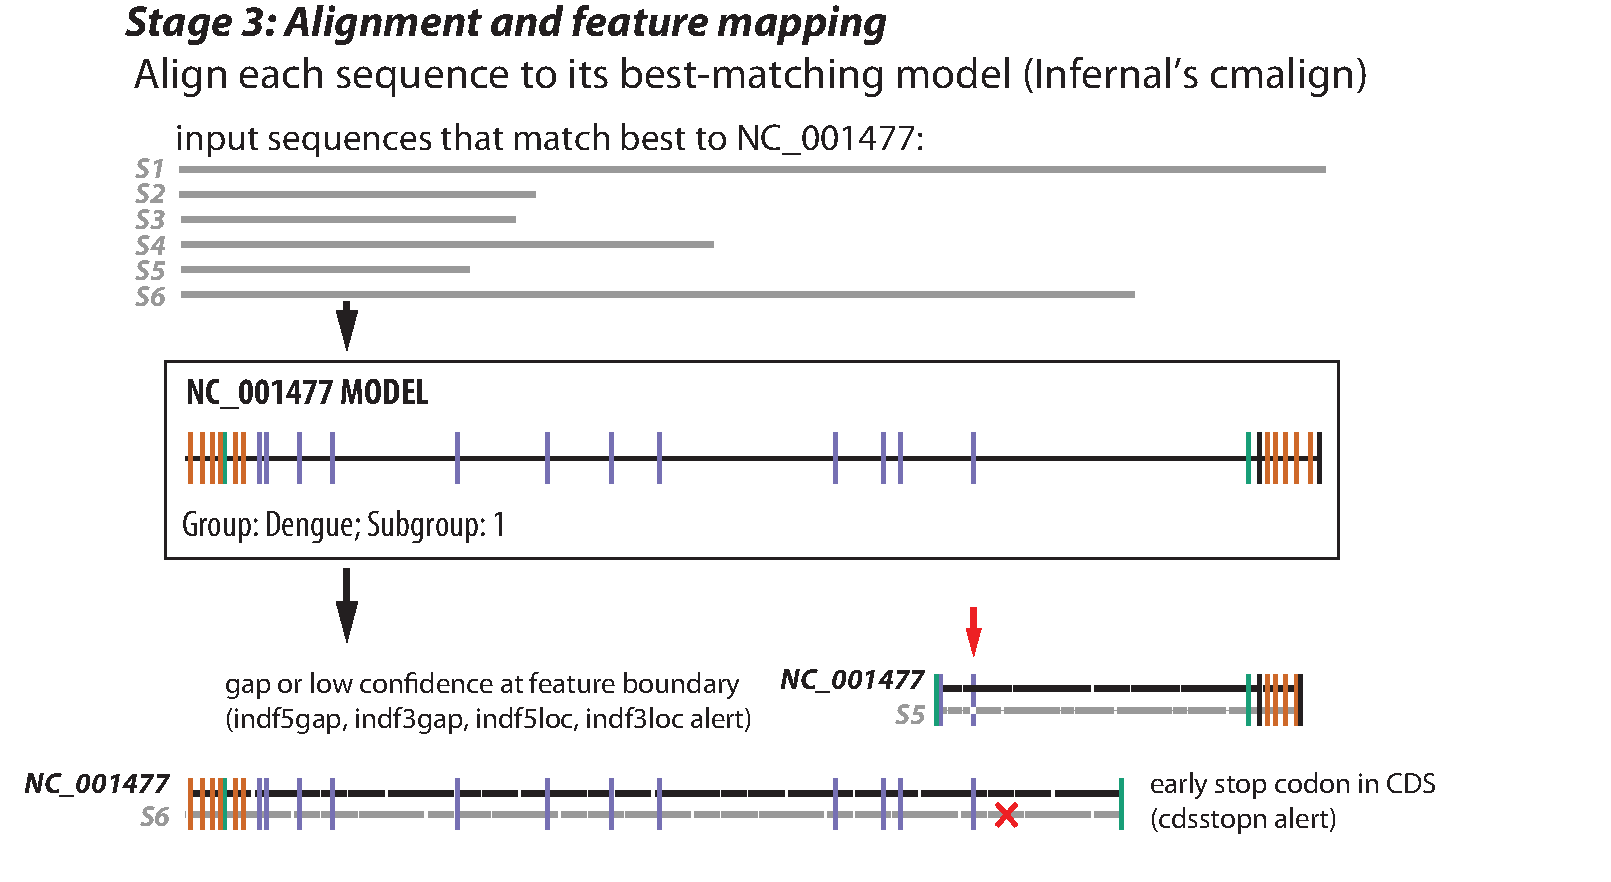
\includegraphics[width=10.5in]{figs/v-annotate-stage3-3}
%\end{center}
%
%\vfill
%\end{slide}
%%%%%%%%%%%%%%%%%%%%%%%%%%%%%%%%%%%%%%%%%%%%%%%%%%%%%%%%%%%%%%%%%%%%%%
\begin{slide}
\begin{center}

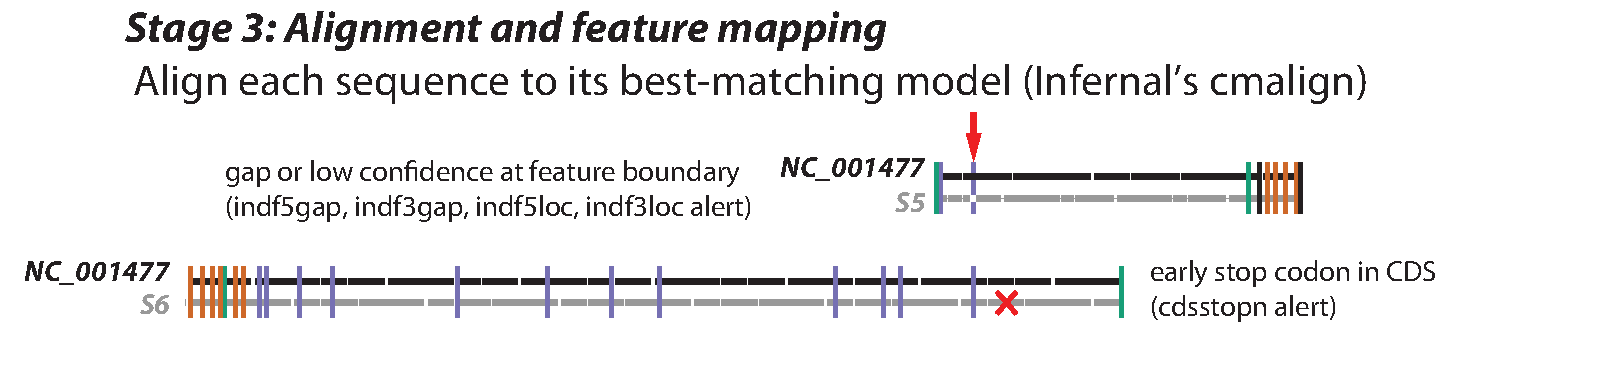
\includegraphics[width=10.5in]{figs/v-annotate-stage3-4}
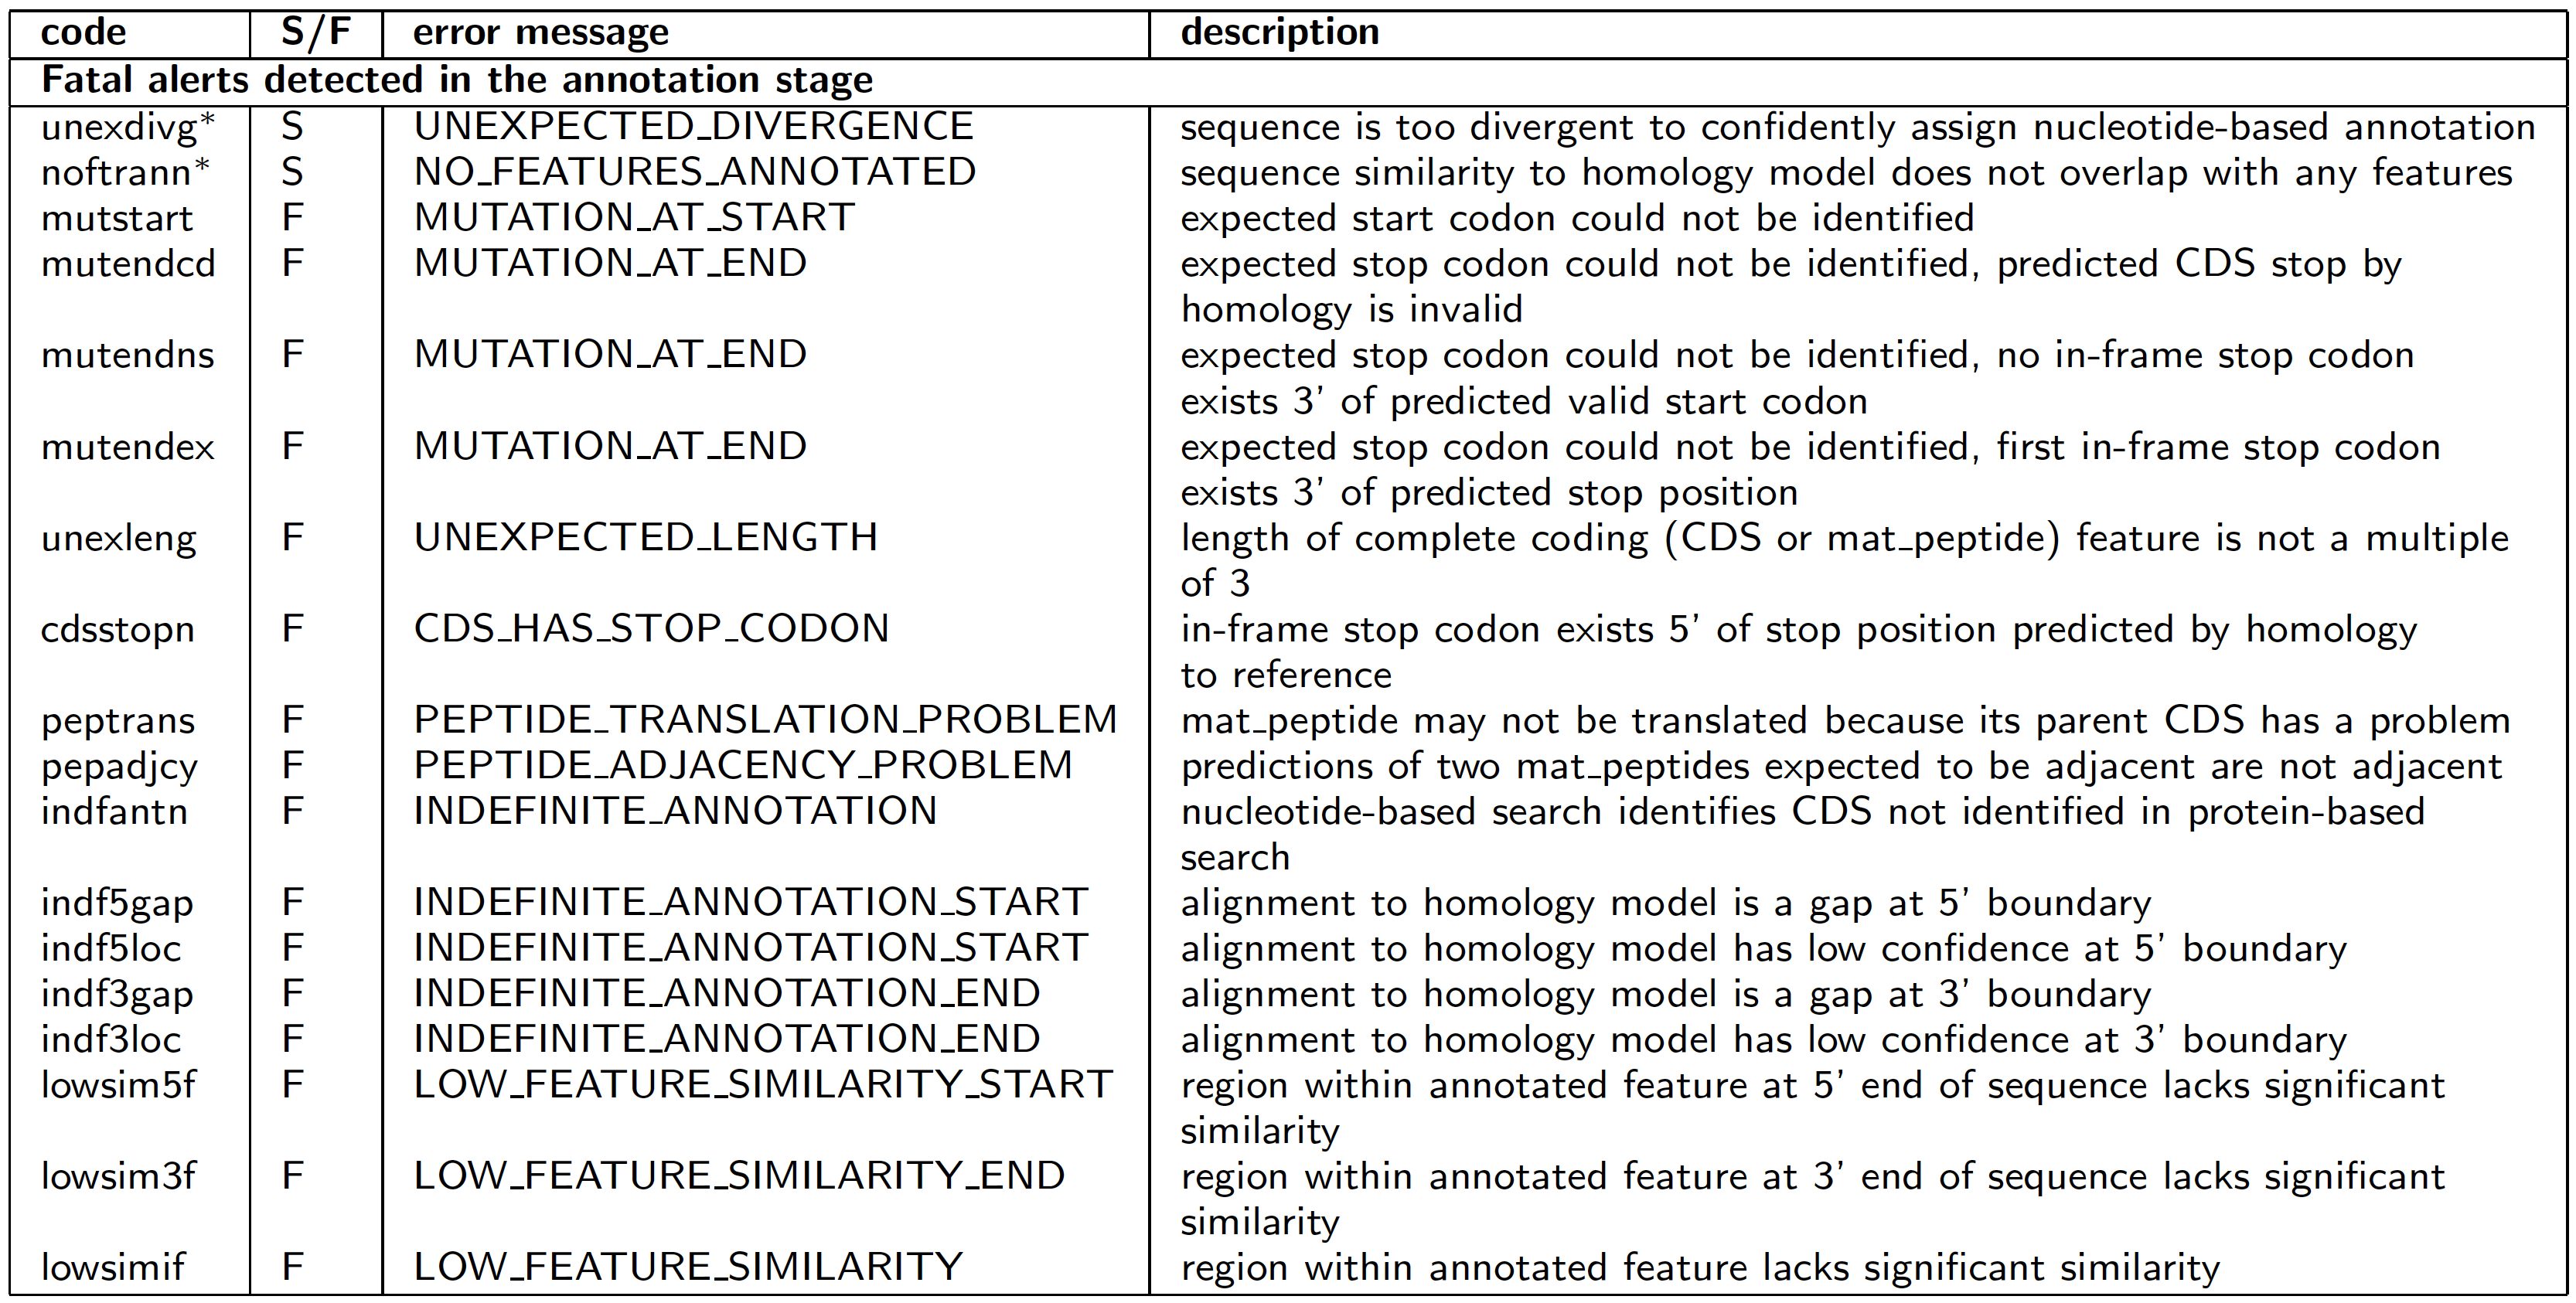
\includegraphics[width=10.5in]{figs/ss-alignment-alert-list}

\end{center}
\vfill
\end{slide}
%%%%%%%%%%%%%%%%%%%%%%%%%%%%%%%%%%%%%%%%%%%%%%%%%%%%%%%%%%%%%%%%%%%%%%
\begin{slide}
\begin{center}

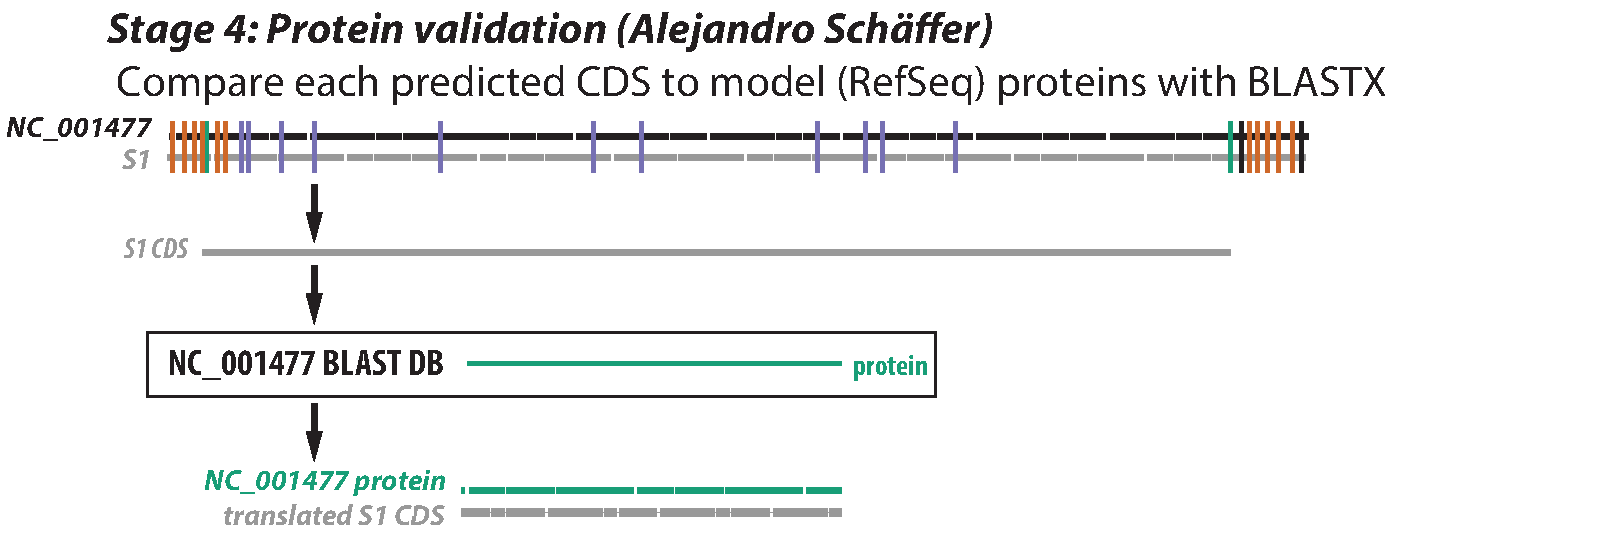
\includegraphics[width=10.5in]{figs/v-annotate-stage4-1}

\end{center}
\vfill
\end{slide}
%%%%%%%%%%%%%%%%%%%%%%%%%%%%%%%%%%%%%%%%%%%%%%%%%%%%%%%%%%%%%%%%%%%%%%
\begin{slide}
\begin{center}

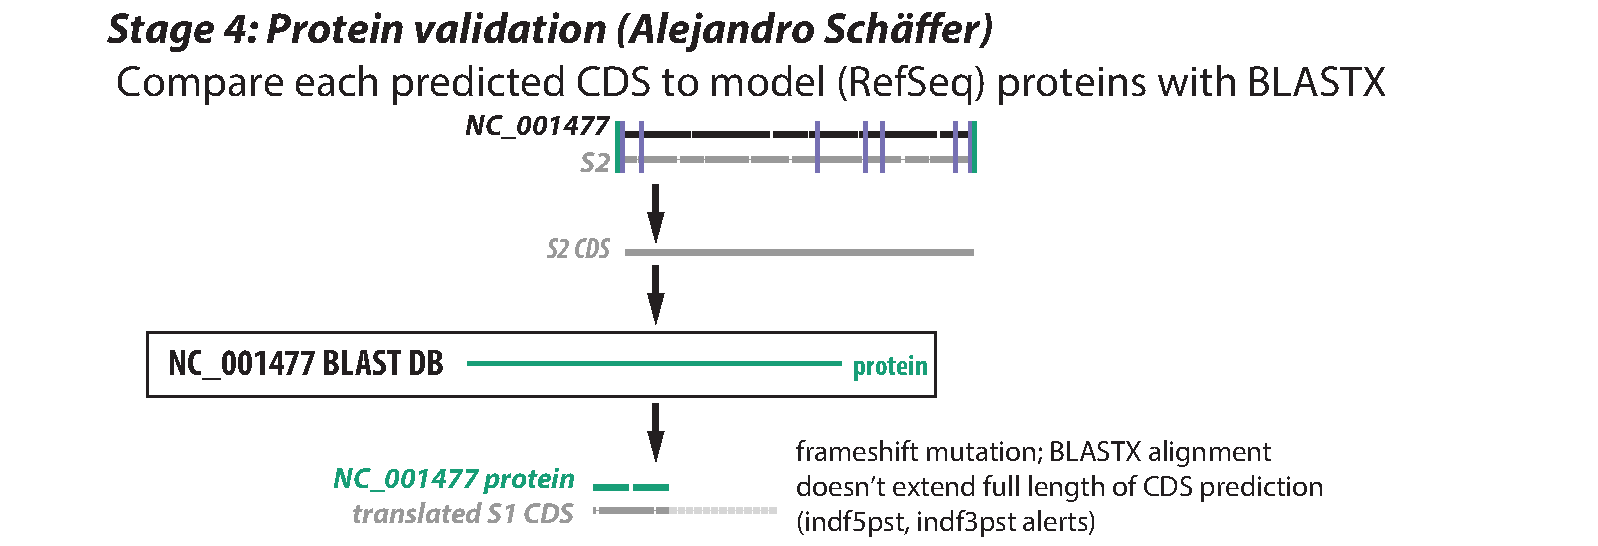
\includegraphics[width=10.5in]{figs/v-annotate-stage4-2}
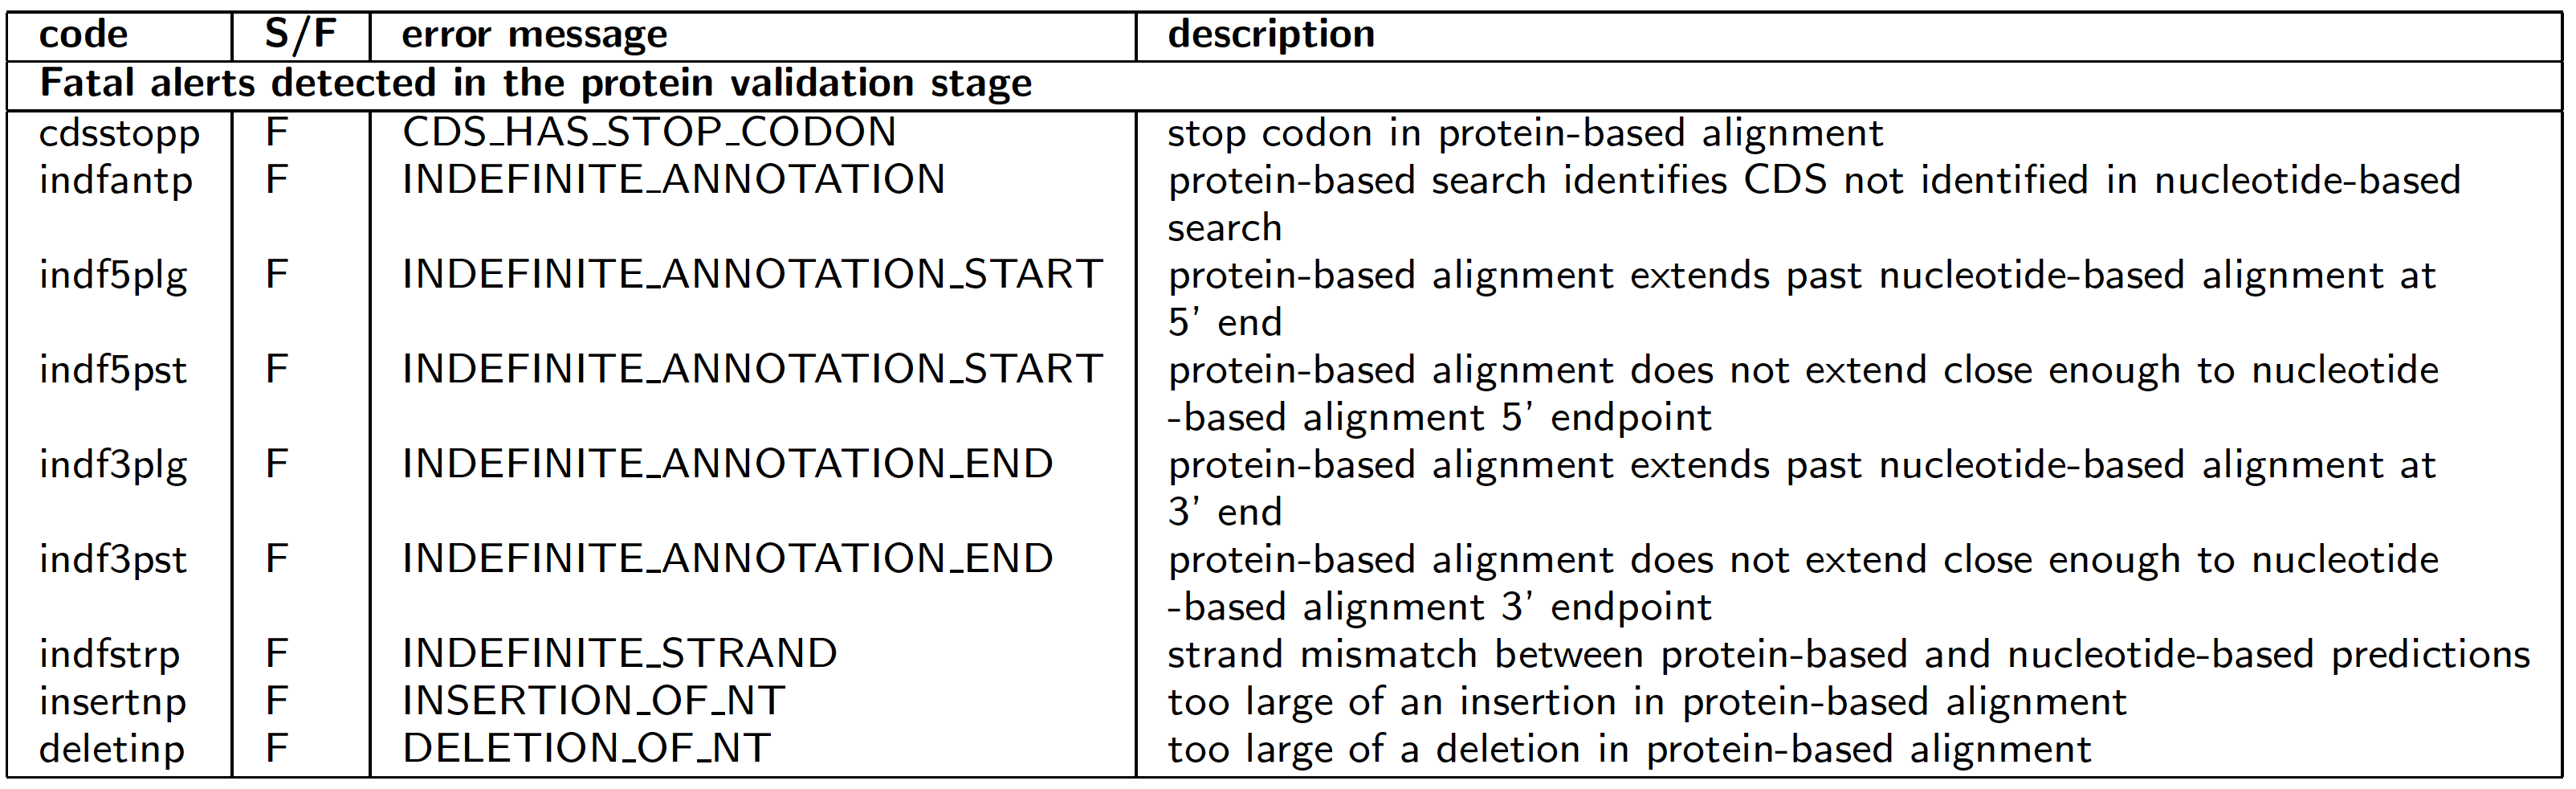
\includegraphics[width=10.5in]{figs/ss-protein-alert-list}

\end{center}
\vfill
\end{slide}
%%%%%%%%%%%%%%%%%%%%%%%%%%%%%%%%%%%%%%%%%%%%%%%%%%%%%%%%%%%%%%%%%%%%%%
\begin{slide}
\begin{center}
\textbf{SARS-CoV-2 sequences in GenBank: Jan 2020 to June 2020}

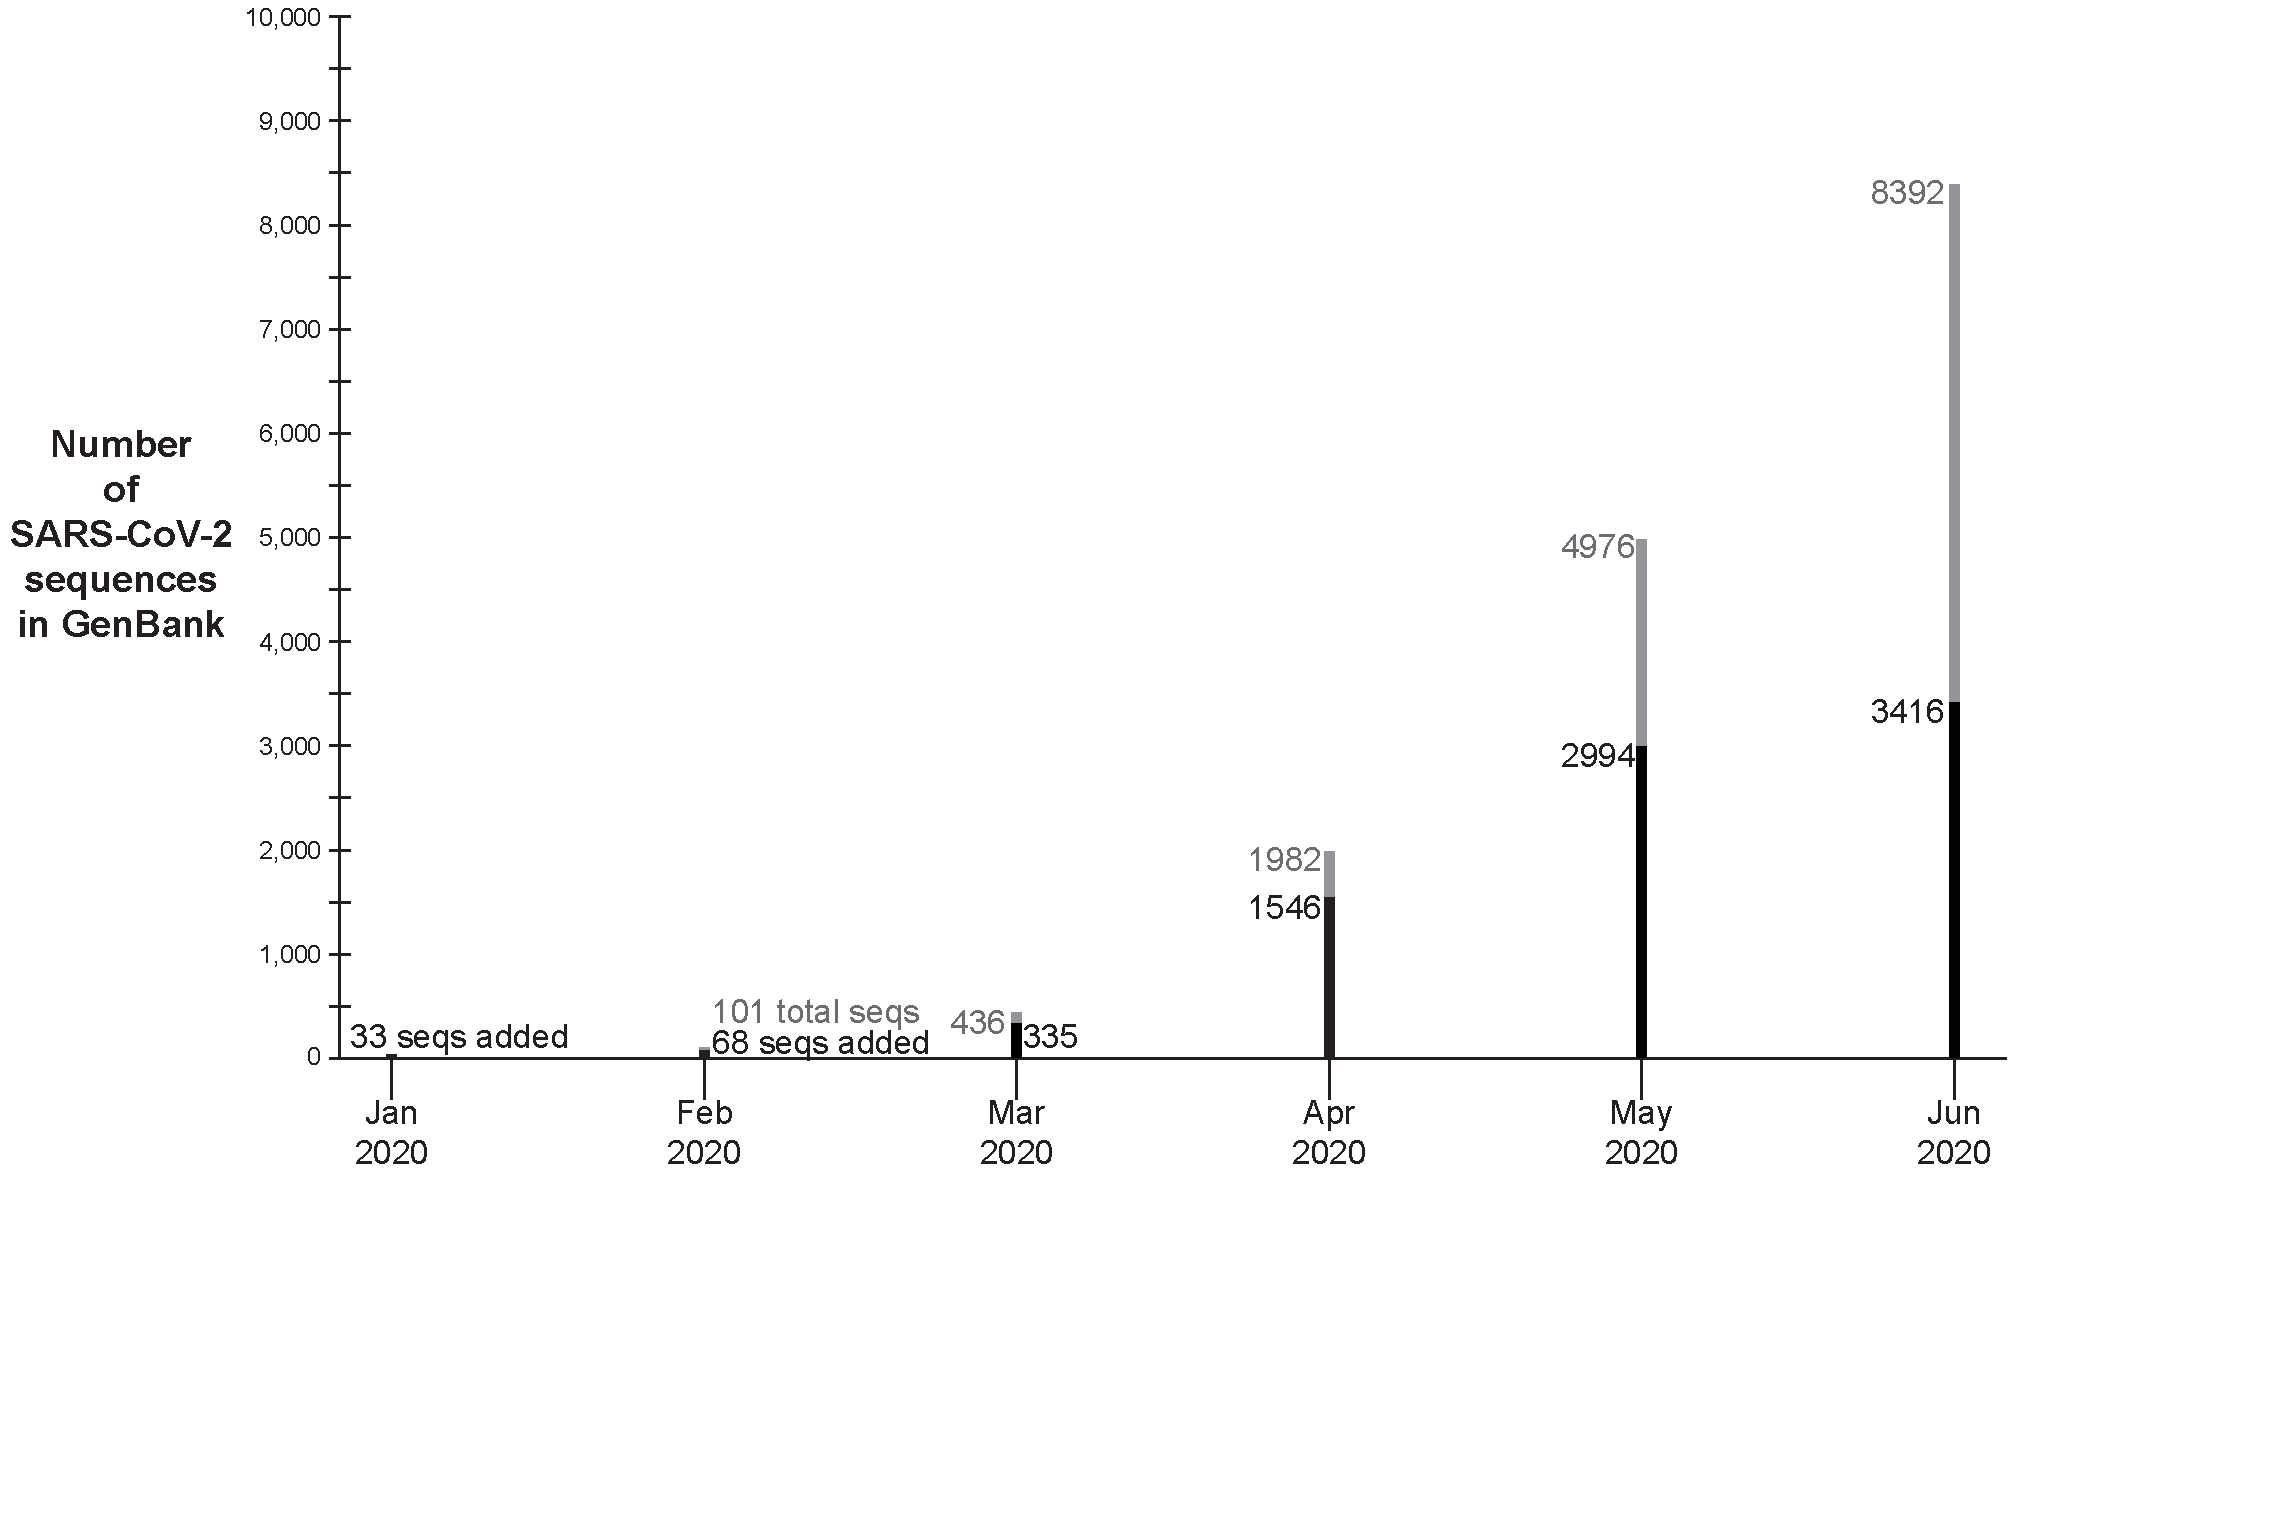
\includegraphics[width=10.5in]{figs/sars-counts-jan2020-may2020-slide1}
\end{center}

\vfill
\end{slide}
%%%%%%%%%%%%%%%%%%%%%%%%%%%%%%%%%%%%%%%%%%%%%%%%%%%%%%%%%%%%%%%%%%%%%%
\begin{slide}
\begin{center}
\textbf{VADR 1.0: functional but slow}

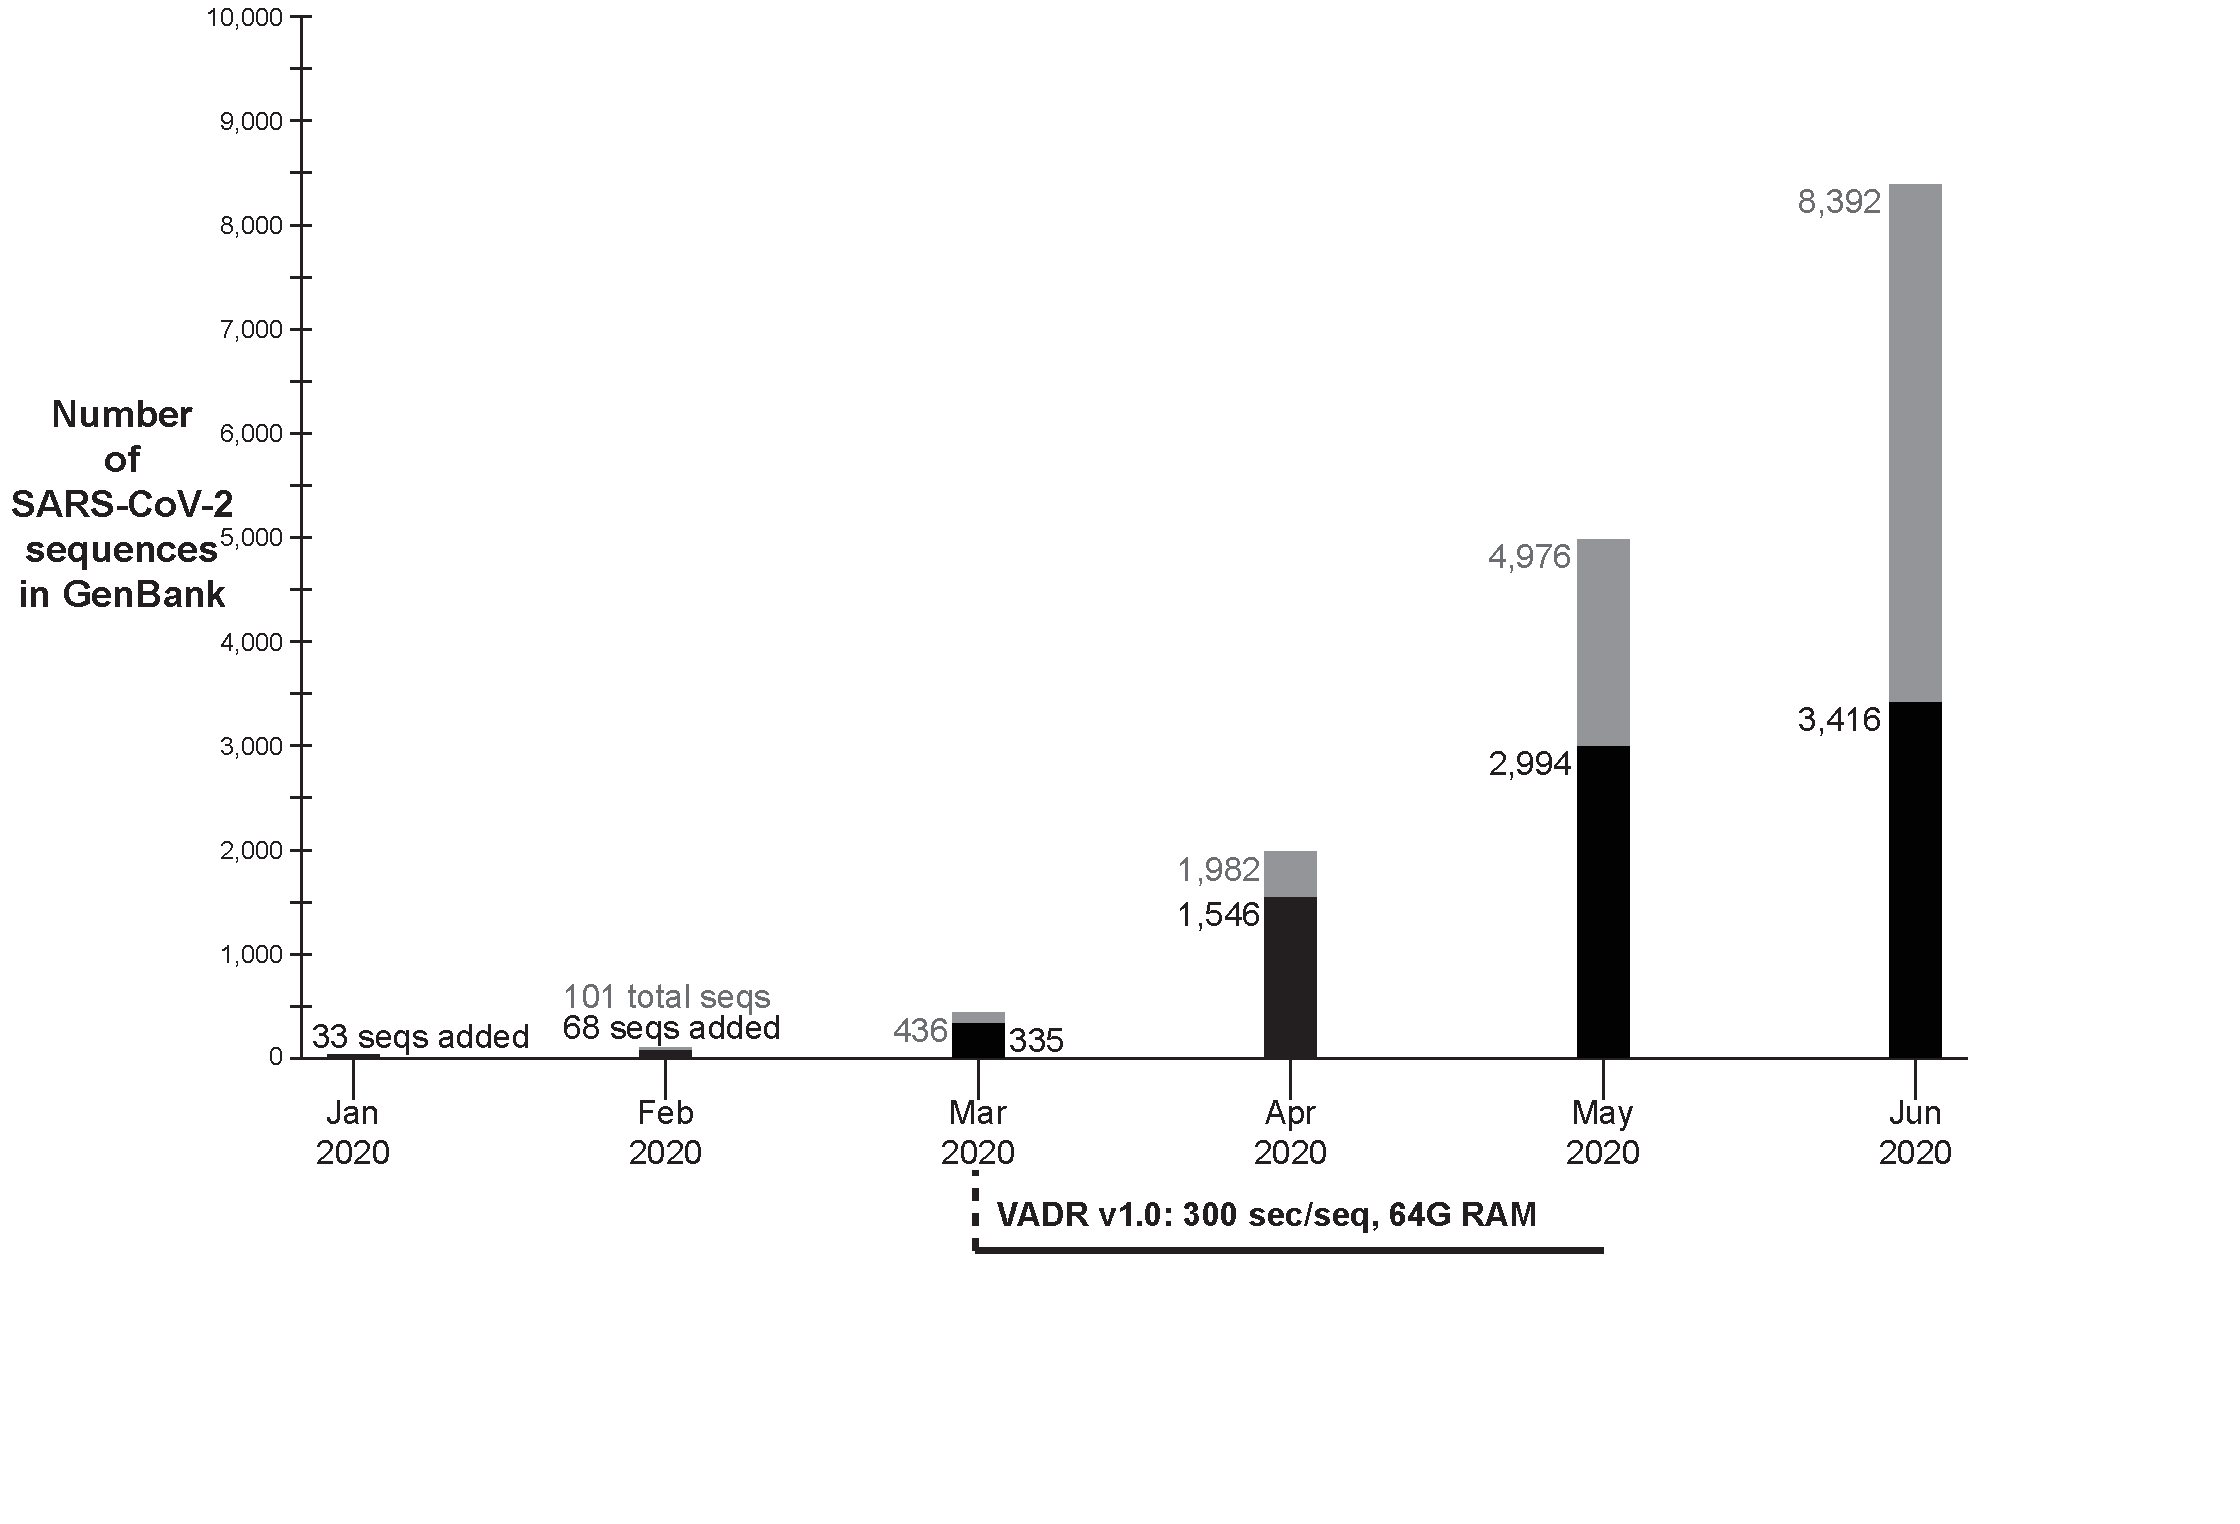
\includegraphics[width=10.5in]{figs/sars-counts-jan2020-may2020-slide2}
\end{center}

\vfill
\end{slide}
%%%%%%%%%%%%%%%%%%%%%%%%%%%%%%%%%%%%%%%%%%%%%%%%%%%%%%%%%%%%%%%%%%%%%%
\begin{slide}
\begin{center}
\textbf{SARS-CoV-2 sequences have a lot of ambiguous nucleotides (Ns)}
\end{center}

\begin{center}
\begin{tabular}{lrr}
            & \% of nucleotides & \% of seqs w/stretch \\
  virus     & that are Ns       & of Ns $>=$ 50 nt     \\ \hline
& & \\
Dengue virus  & 0.0037\%        & 0.0070\%             \\
& & \\                    
Norovirus     & 0.296\%         & 0.628\%             \\
& & \\                    
\textcolor{red}{SARS-CoV-2}    & \textcolor{red}{1.12\%}          & \textcolor{red}{\emph{26.4\%}}       \\
\end{tabular}
\end{center}
\vfill

\vfill
\end{slide}
%%%%%%%%%%%%%%%%%%%%%%%%%%%%%%%%%%%%%%%%%%%%%%%%%%%%%%%%%%%%%%%%%%%%%%
\begin{slide}
\begin{center}
\textbf{SARS-CoV-2 sequences have a lot of ambiguous nucleotides (Ns)}
\end{center}

\begin{center}
\begin{tabular}{lrr}
            & \% of nucleotides & \% of seqs w/stretch \\
  virus     & that are Ns       & of Ns $>=$ 50 nt     \\ \hline
& & \\
Dengue virus  & 0.0037\%        & 0.0070\%             \\
& & \\                    
Norovirus     & 0.296\%         & 0.628\%             \\
& & \\                    
\textcolor{red}{SARS-CoV-2}    & \textcolor{red}{1.12\%}          & \textcolor{red}{\emph{26.4\%}}       \\
\end{tabular}
\end{center}
\vfill

\begin{center}
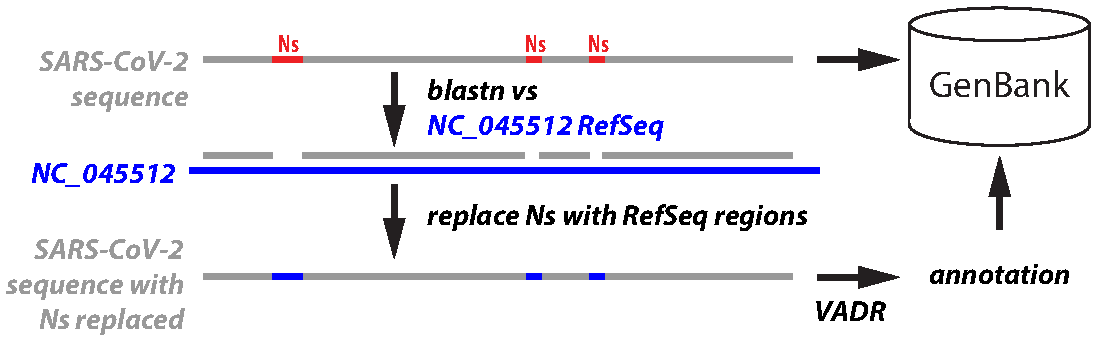
\includegraphics[width=10.5in]{figs/vadr-r-option}
\end{center}

%\begin{itemize}
%\item
%  N-rich sequences fail VADR because it relies on global sequence similarity
%\item
%  New strategy in VADR 1.1:
%  \begin{itemize}
%    \item identifies stretches of Ns of expected length
%    \item replaces Ns with the corresponding RefSeq sequence
%    \item validates and annotates sequences with Ns replaced
%    \item puts Ns back in prior to GenBank submission
%  \end{itemize}
%\end{itemize}
%
\vfill
\end{slide}
%%%%%%%%%%%%%%%%%%%%%%%%%%%%%%%%%%%%%%%%%%%%%%%%%%%%%%%%%%%%%%%%%%%%%%
\begin{slide}
\begin{center}
%\textbf{SARS-CoV-2 sequences (especially early ones) are all highly
%  similar to the reference (typically $>$ 99.5\%)}
\large{\textbf{VADR 1.1 exploits high similarity (typically $>$ 99.5\%) \\ of SARS-CoV-2 sequences to the RefSeq}}
\end{center}

\begin{itemize}
  \item blastn replaces hmmer3 in classification and coverage determination stages
  \item max ungapped blastn alignment region \emph{seeds} the cmalign alignment
\end{itemize}

\begin{center}
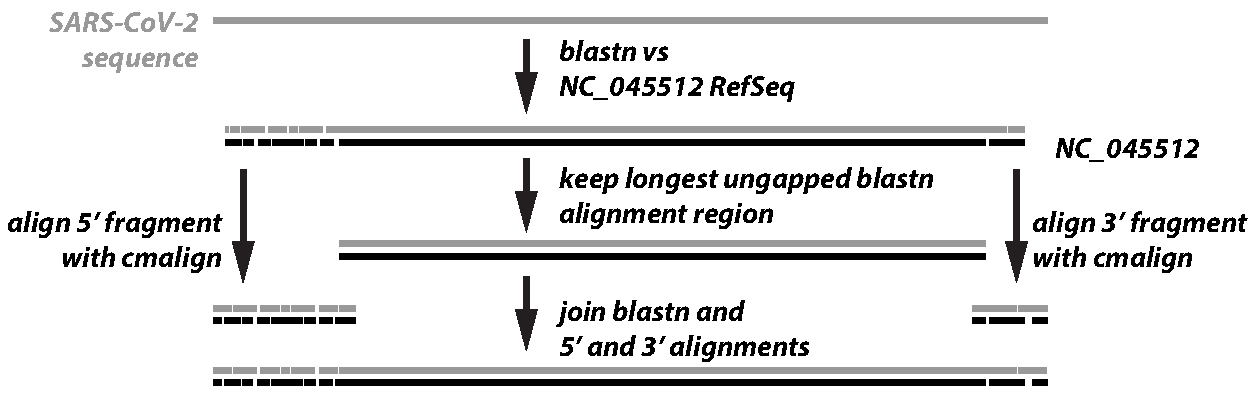
\includegraphics[width=10.5in]{figs/vadr-s-option}
\end{center}

\vfill
\end{slide}
%%%%%%%%%%%%%%%%%%%%%%%%%%%%%%%%%%%%%%%%%%%%%%%%%%%%%%%%%%%%%%%%%%%%%%
\begin{slide}
\begin{center}
\large{\textbf{VADR 1.1: 150X speedup on typical sequences}}

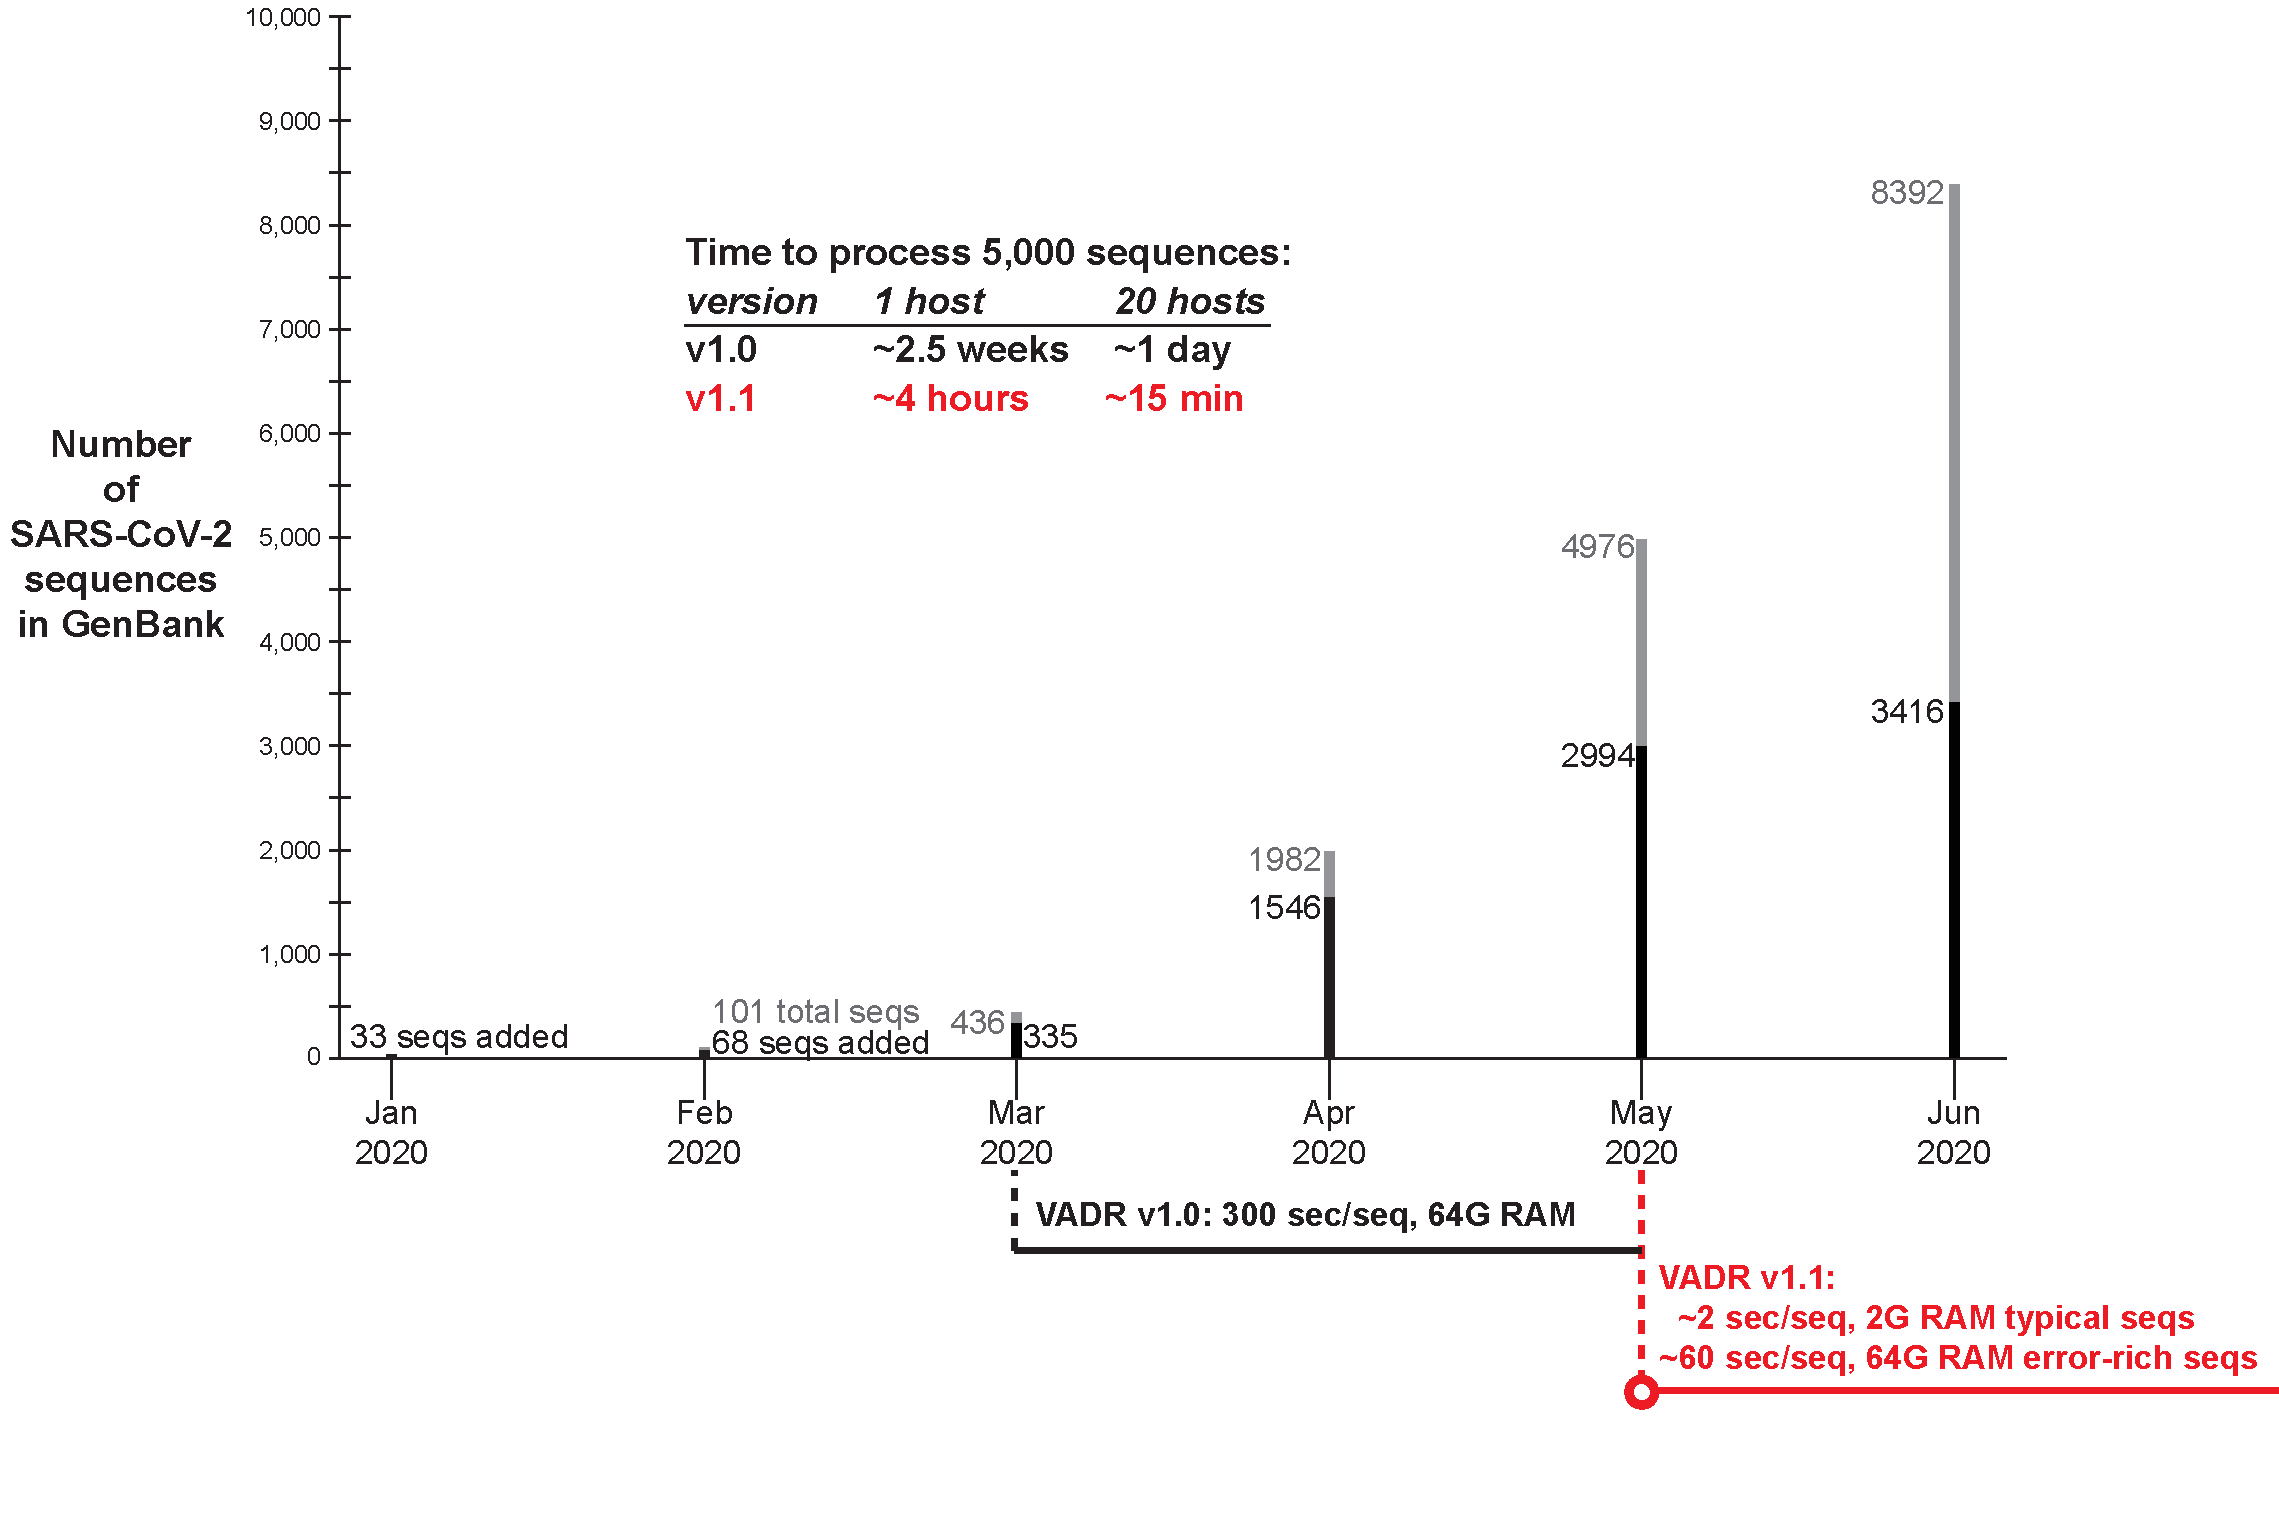
\includegraphics[width=10.5in]{figs/sars-counts-jan2020-may2020-slide3}
\end{center}

\vfill
\end{slide}
%%%%%%%%%%%%%%%%%%%%%%%%%%%%%%%%%%%%%%%%%%%%%%%%%%%%%%%%%%%%%%%%%%%%%%
\begin{slide}
\begin{center}
\large{\textbf{VADR 1.1: 150X speedup on typical sequences}}

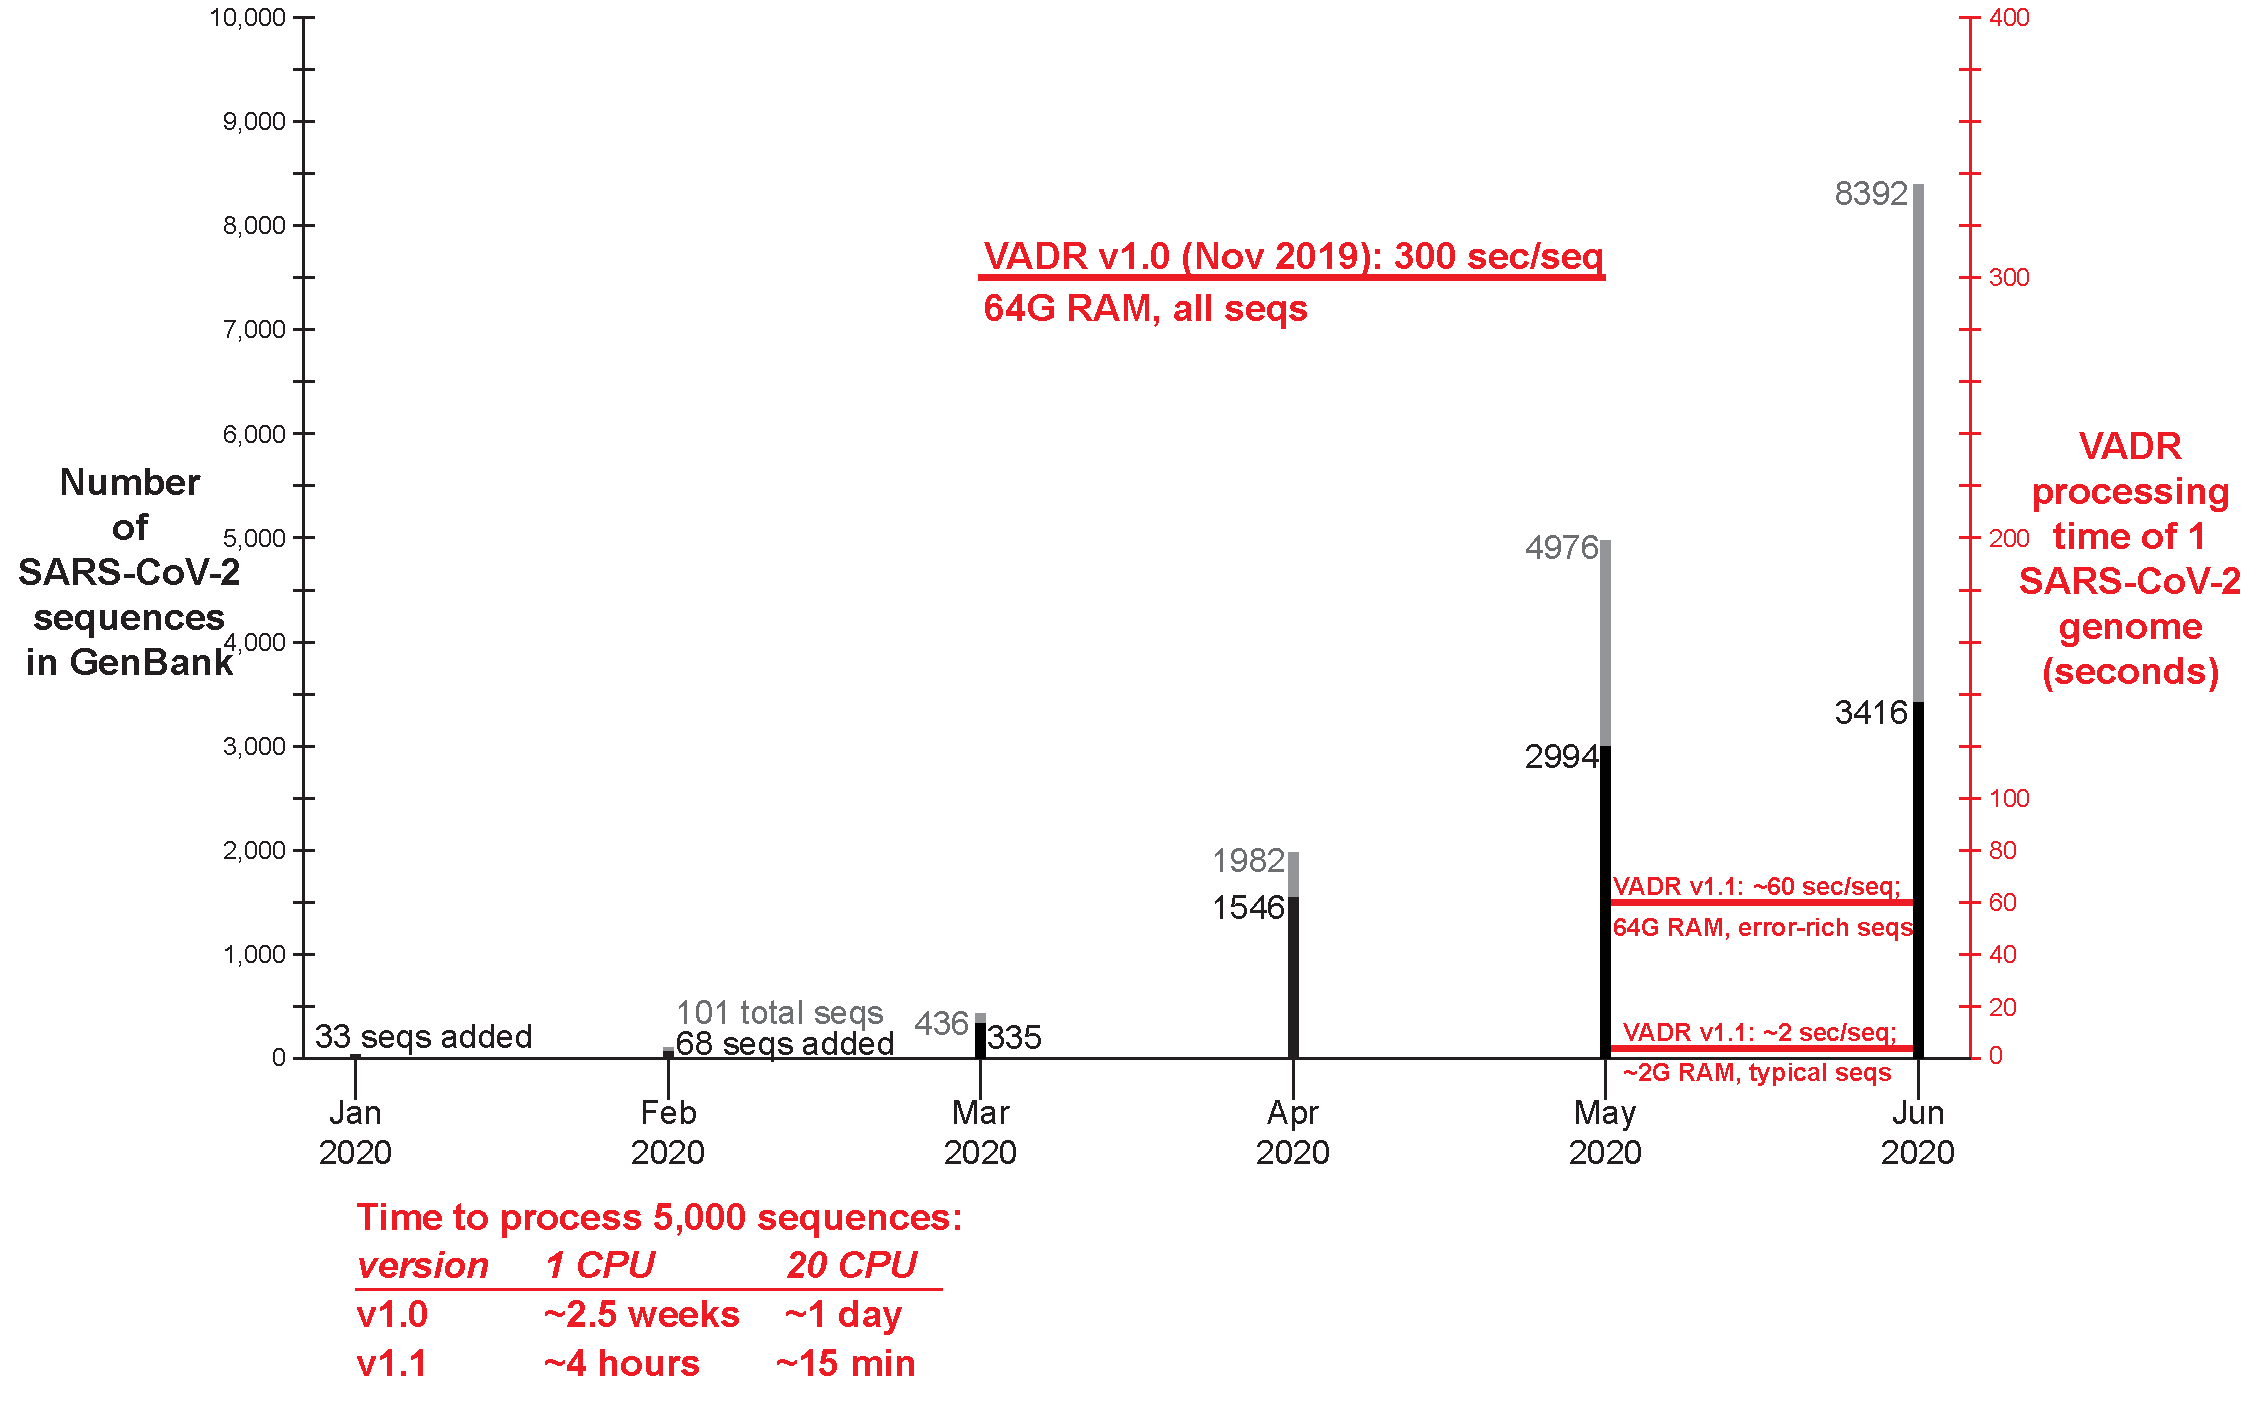
\includegraphics[width=10.5in]{figs/sars-counts-jan2020-may2020-slide4}
\end{center}

\vfill
\end{slide}
%%%%%%%%%%%%%%%%%%%%%%%%%%%%%%%%%%%%%%%%%%%%%%%%%%%%%%%%%%%%%%%%%%%%%%
\begin{slide}
\begin{center}
\textbf{Sequence volume increased dramatically in 2021}

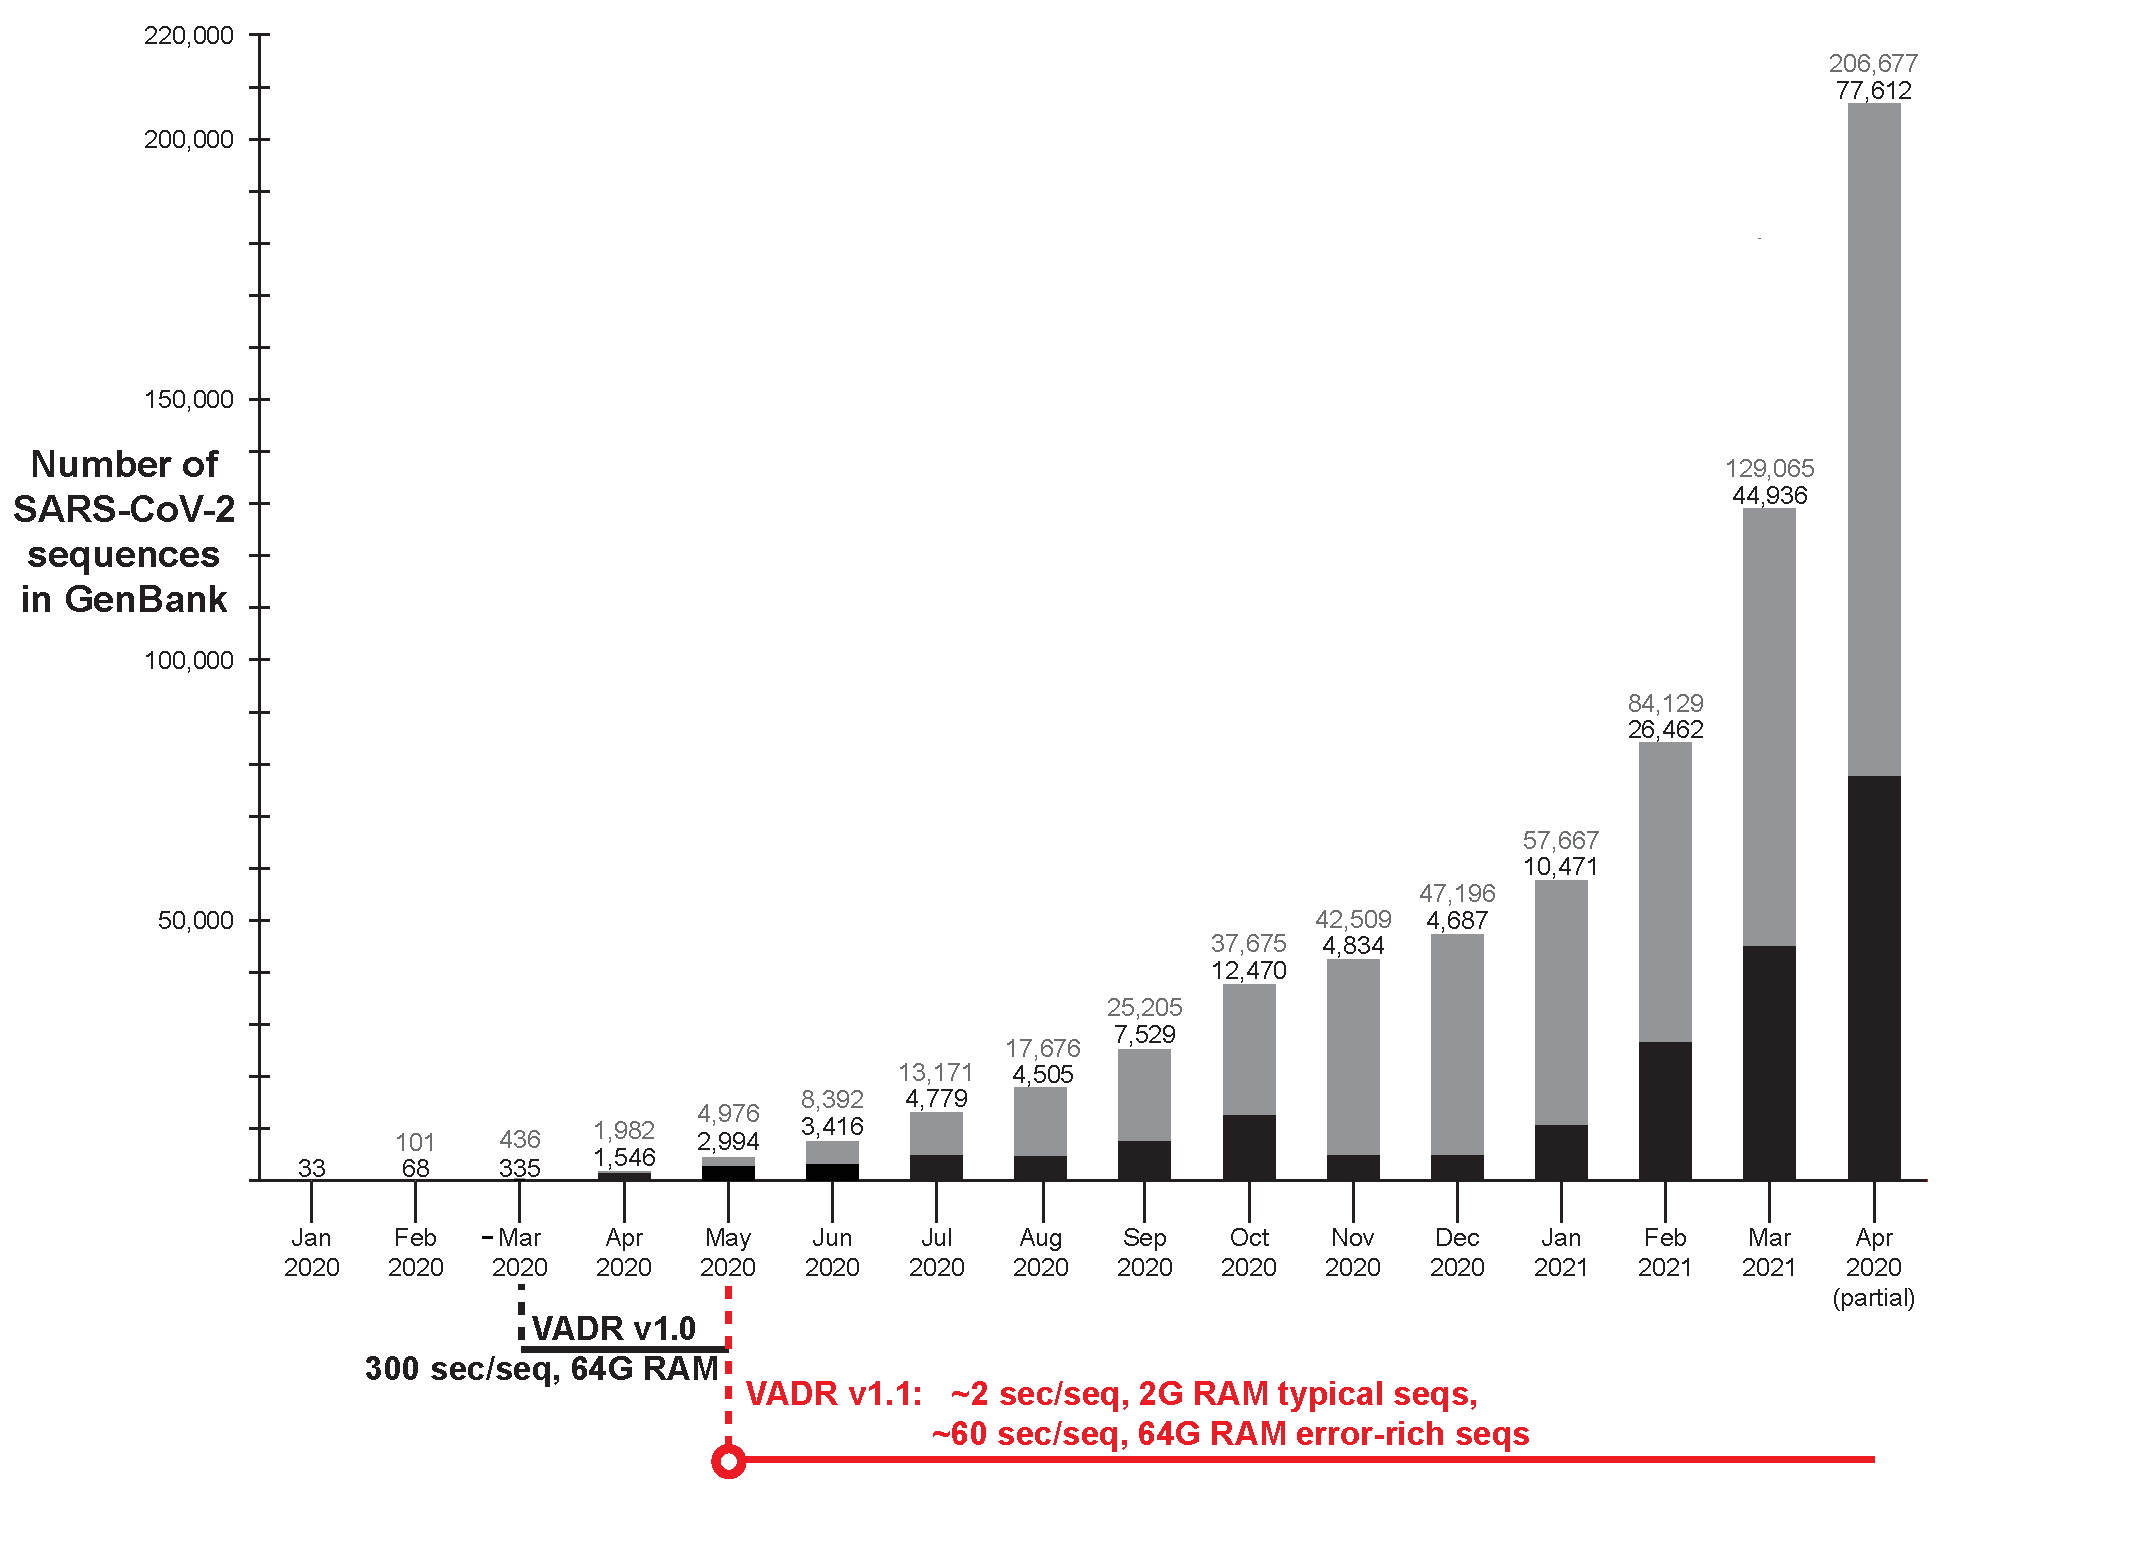
\includegraphics[width=10.25in]{figs/sars-counts-jan2020-apr2021-slide1}
\end{center}

\vfill
\end{slide}
%%%%%%%%%%%%%%%%%%%%%%%%%%%%%%%%%%%%%%%%%%%%%%%%%%%%%%%%%%%%%%%%%%%%%%
\begin{slide}
\begin{center}
\large{\textbf{Speed and memory bottleneck in VADR 1.1 is cmalign}}
\end{center}

\begin{itemize}
\item VADR 1.2 replaces cmalign with glsearch ('glocal' alignment)
  \begin{itemize}
  \item lower memory requirement (2G max) opens door for multi-threading
%  \item input file is split into chunks
%    \begin{itemize}
%    \item each chunk processed independently in parallel on one of 8 CPUs
%    \item further reduces memory requirement for large input files \\ (dependent on chunk size
%      instead of input file size)
%    \end{itemize}
  \end{itemize}
\end{itemize}

\begin{center}
\includegraphics[width=10.5in]{figs/vadr-1p2-multithreading}
\end{center}
  
\vfill
\end{slide}
%%%%%%%%%%%%%%%%%%%%%%%%%%%%%%%%%%%%%%%%%%%%%%%%%%%%%%%%%%%%%%%%%%%%%%
\begin{slide}
\begin{center}
\textbf{VADR v1.2 is about 10X faster than v1.1}

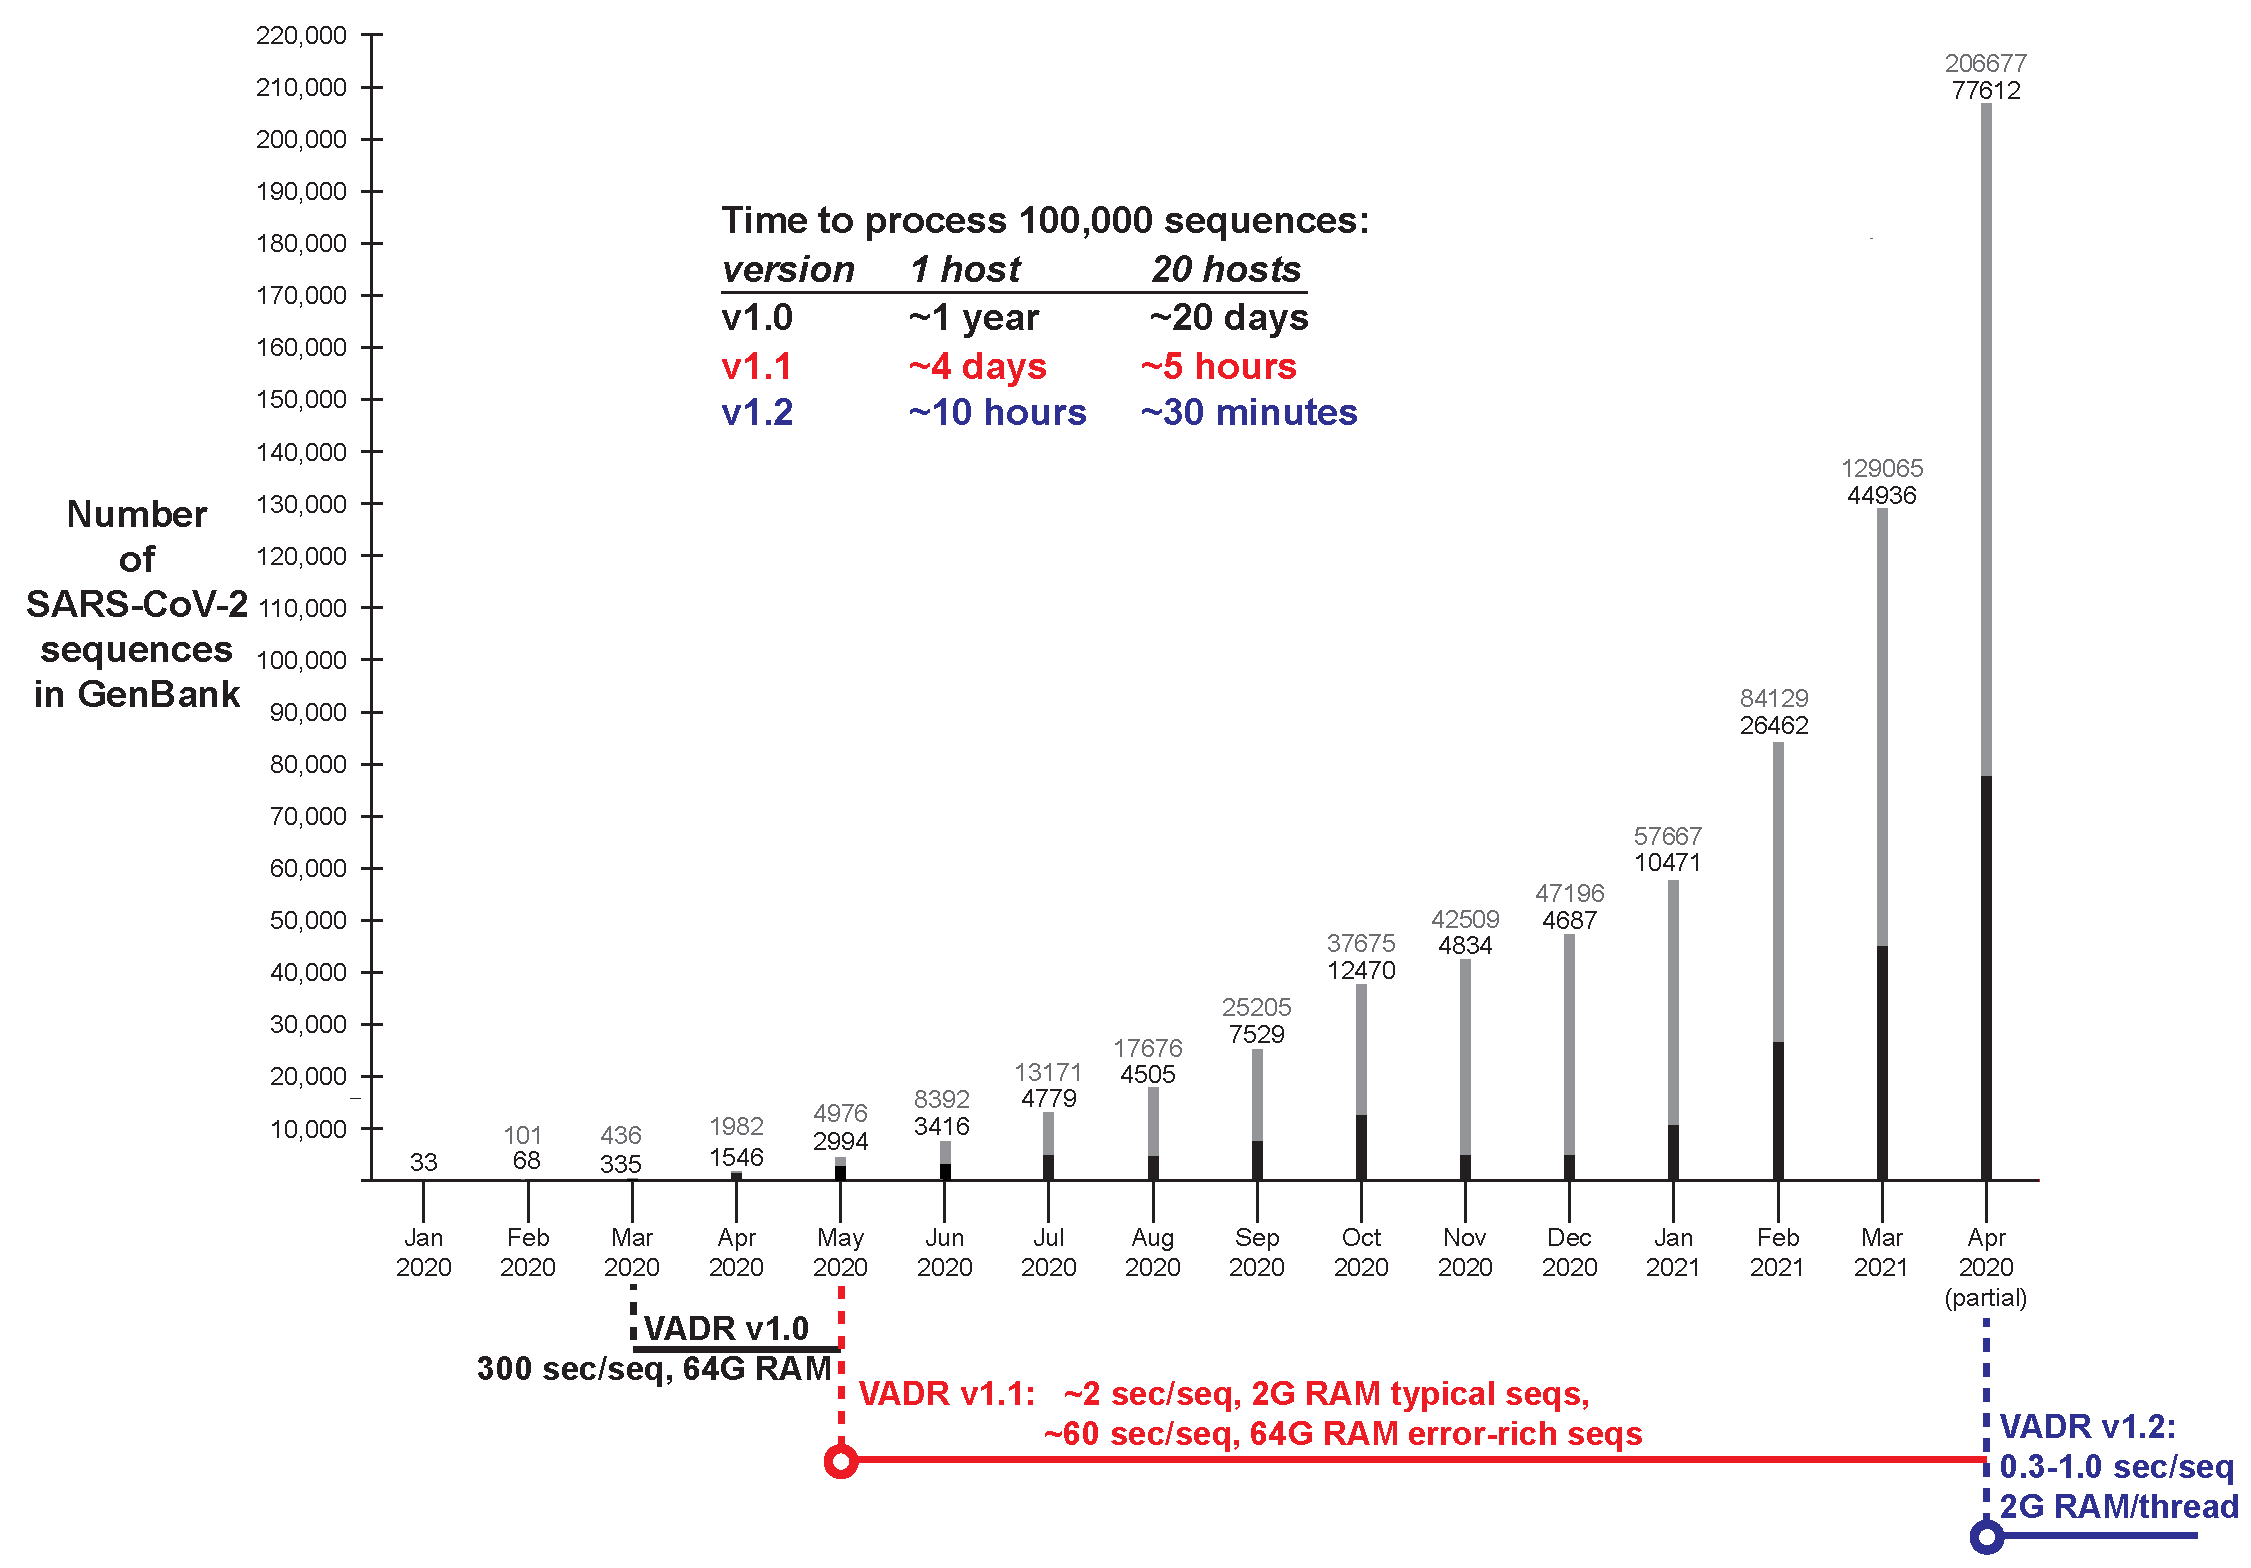
\includegraphics[width=10.25in]{figs/sars-counts-jan2020-apr2021-slide2}
\end{center}

\vfill
\end{slide}
%%%%%%%%%%%%%%%%%%%%%%%%%%%%%%%%%%%%%%%%%%%%%%%%%%%%%%%%%%%%%%%%%%%%%%
\begin{slide}
\begin{center}
\textbf{GenBank is now better prepared for large sequence submissions}

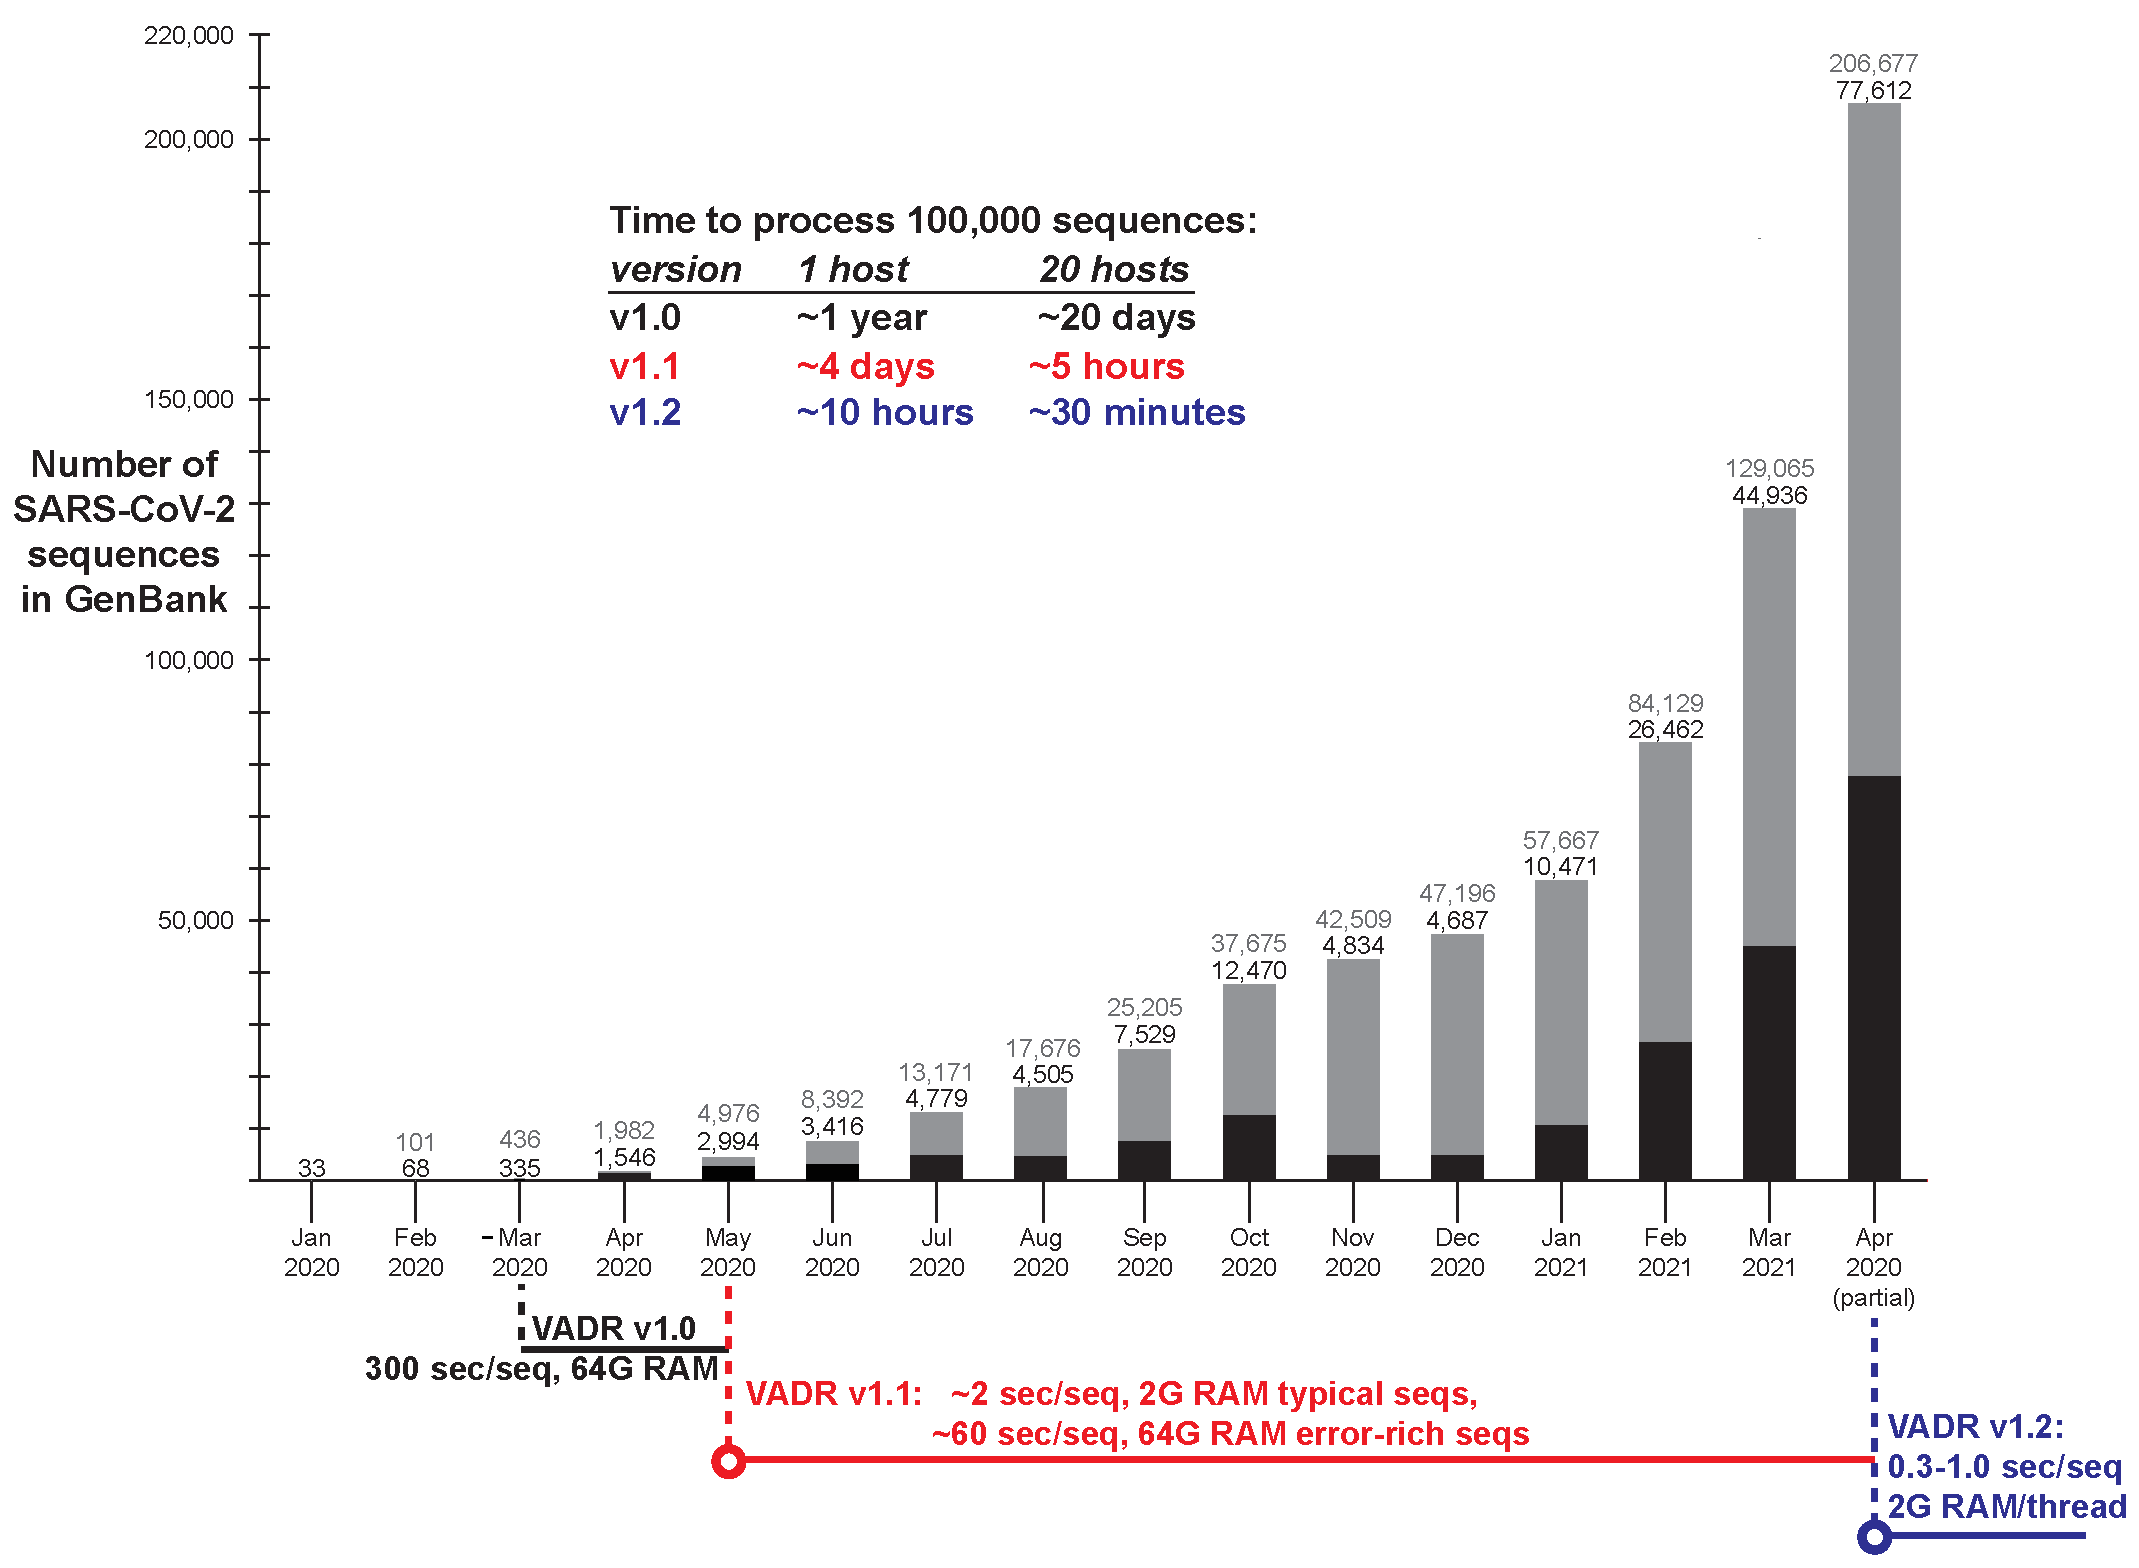
\includegraphics[width=10.25in]{figs/sars-counts-jan2020-apr2021-slide3}
\end{center}

\vfill
\end{slide}
%%%%%%%%%%%%%%%%%%%%%%%%%%%%%%%%%%%%%%%%%%%%%%%%%%%%%%%%%%%%%%%%%%%%%%
%\begin{slide}
%\begin{center}
%\large{\textbf{Besides getting faster, VADR has improved in other ways}}
%
%\small
%\begin{itemize}
%\item B.1.1.7 variant
%  \begin{itemize}
%    \item Dec 29, 2020: first B.1.1.7 sequence submitted to GenBank
%    \item Jan 8,  2021: B.1.1.7 VADR model available for download (10 seqs in GenBank)
%  \end{itemize}
%\item Feb 12, 2021: VADR 1.1.3
%  \begin{itemize}
%    \item Review of common, supported mutations led to flexibility to allow errors in ORF8 (or any
%  specified CDS) 
%  \end{itemize}
%\item Apr 12, 2021: B.1.525 VADR model (49nt deletion that removes a stem loop)
%\end{itemize}
%\end{center}
%
%\vfill
%\end{slide}
%%%%%%%%%%%%%%%%%%%%%%%%%%%%%%%%%%%%%%%%%%%%%%%%%%%%%%%%%%%%%%%%%%%%%%%%%
\begin{slide}
\begin{center}
\textbf{Besides getting faster, VADR has improved in other ways}

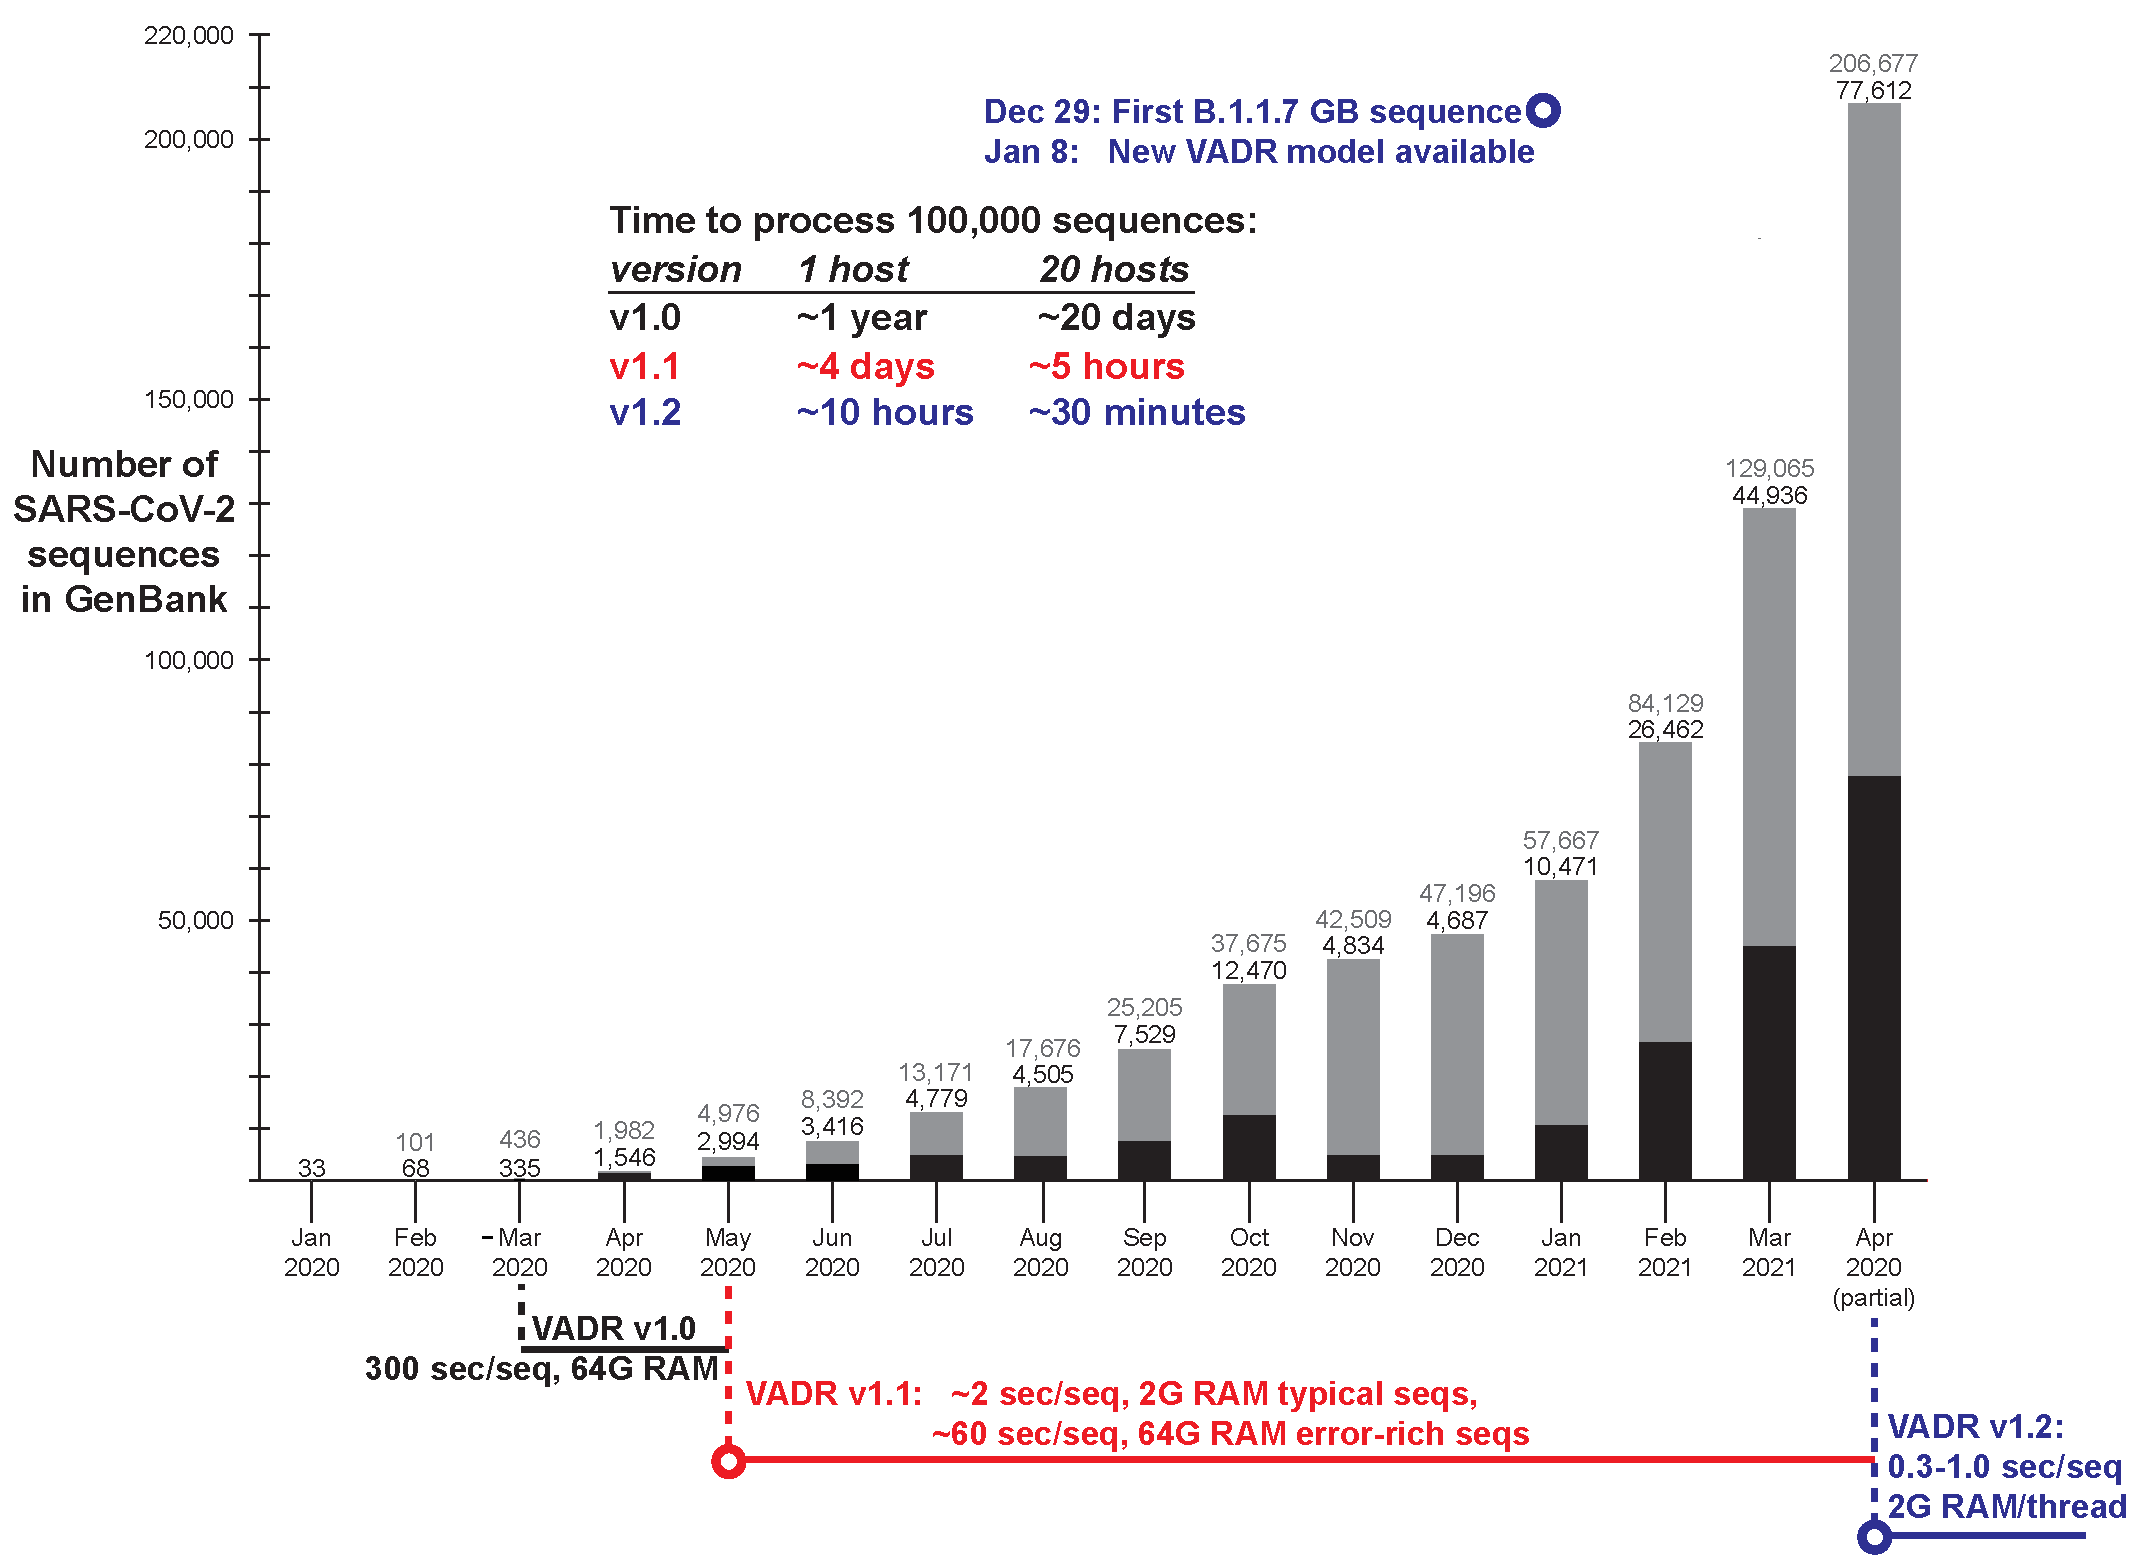
\includegraphics[width=10.25in]{figs/sars-counts-jan2020-apr2021-slide4}

\end{center}

\vfill
\end{slide}
%%%%%%%%%%%%%%%%%%%%%%%%%%%%%%%%%%%%%%%%%%%%%%%%%%%%%%%%%%%%%%%%%%%%%%
\begin{slide}
\begin{center}
\textbf{Besides getting faster, VADR has improved in other ways}

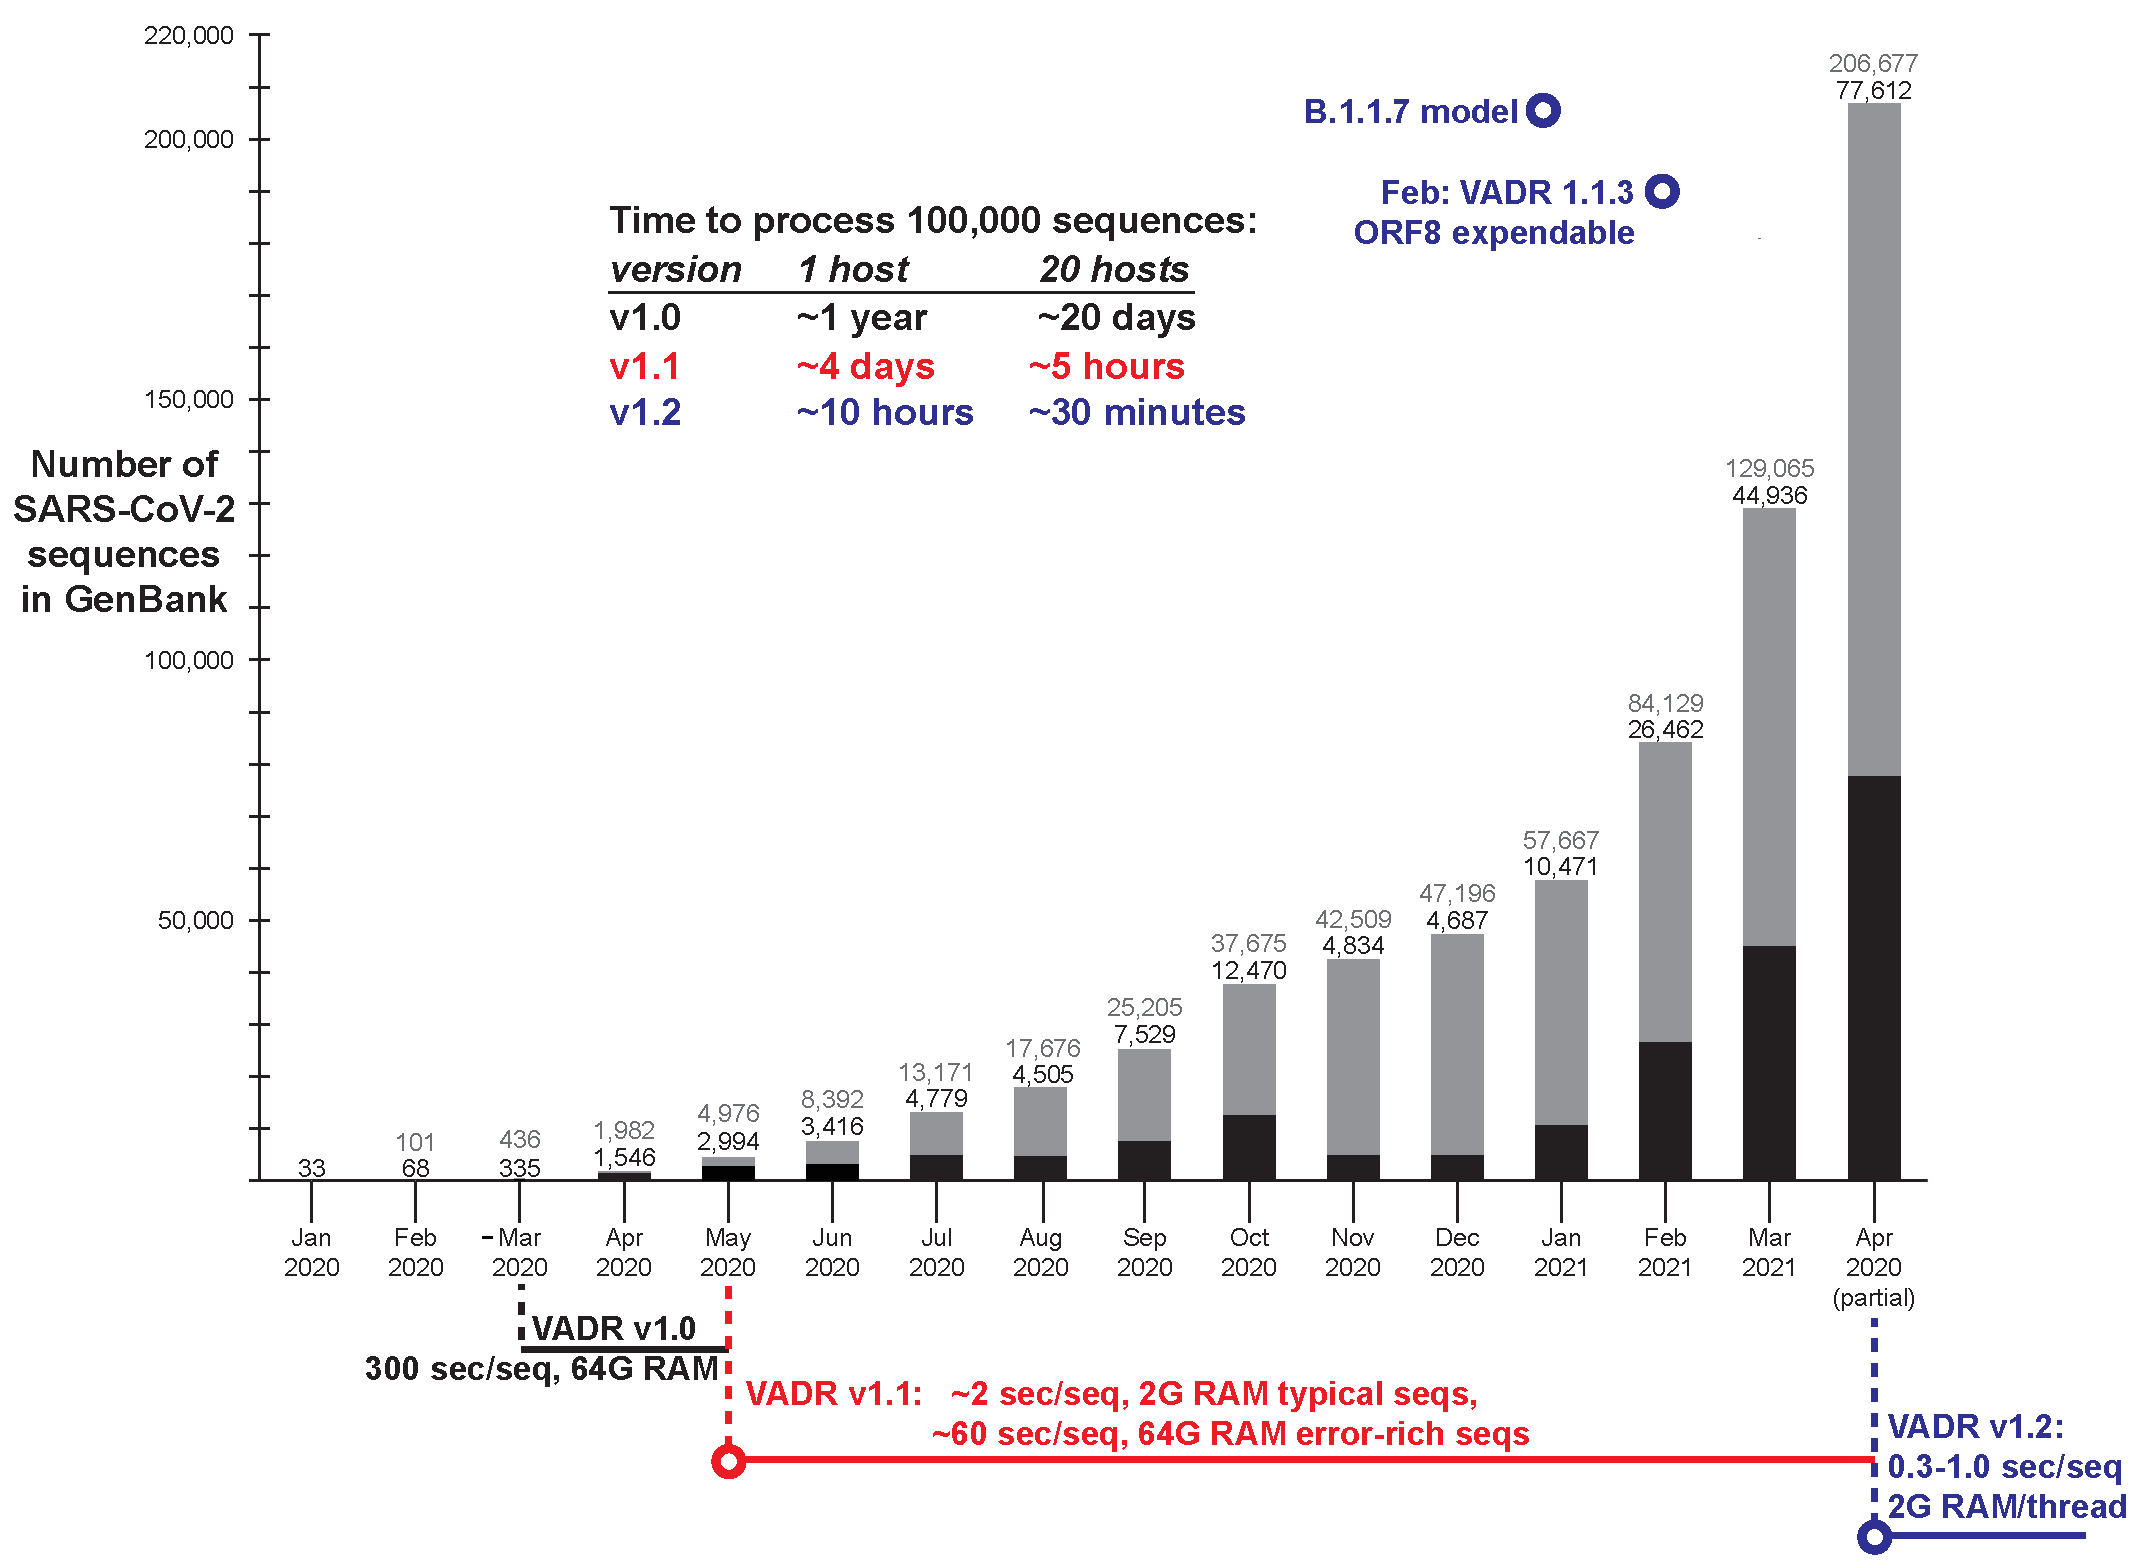
\includegraphics[width=10.25in]{figs/sars-counts-jan2020-apr2021-slide5}

\end{center}

\vfill
\end{slide}
%%%%%%%%%%%%%%%%%%%%%%%%%%%%%%%%%%%%%%%%%%%%%%%%%%%%%%%%%%%%%%%%%%%%%%
\begin{slide}
\begin{center}
\textbf{Besides getting faster, VADR has improved in other ways}

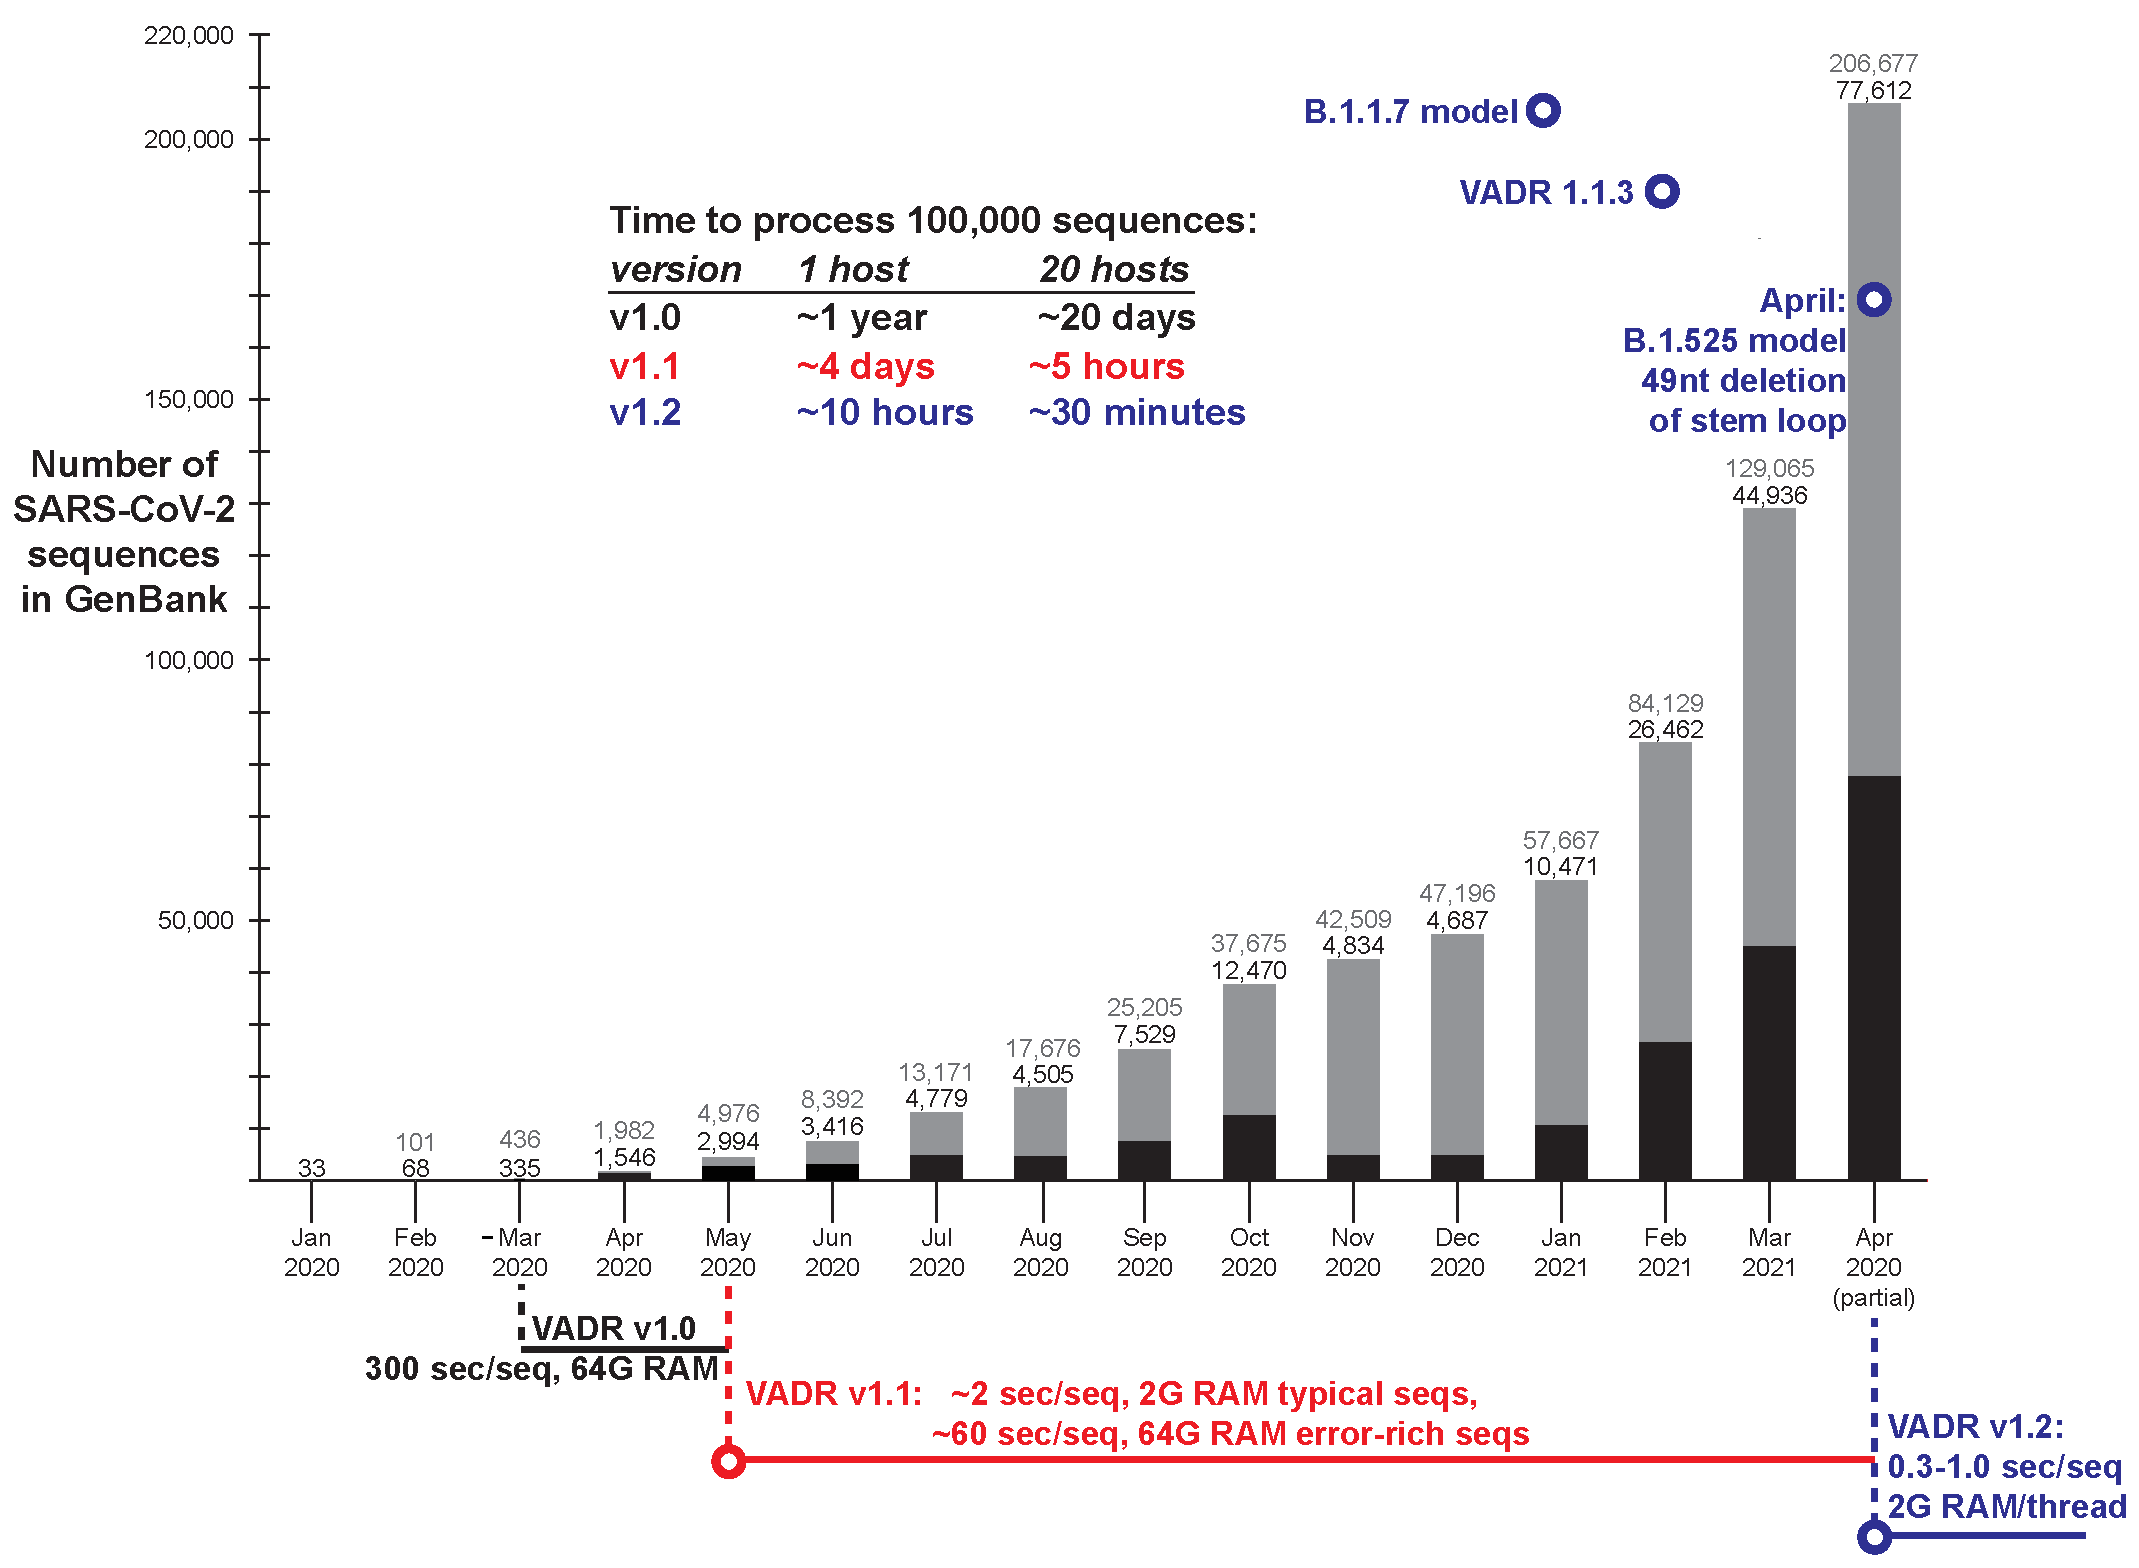
\includegraphics[width=10.25in]{figs/sars-counts-jan2020-apr2021-slide6}

\end{center}

\vfill
\end{slide}
%%%%%%%%%%%%%%%%%%%%%%%%%%%%%%%%%%%%%%%%%%%%%%%%%%%%%%%%%%%%%%%%%%%%%%
%\begin{slide}
%\begin{center}
%\Large{\textbf{We verify VADR passes new SARS-CoV-2 lineages}}
%
%\small
%\begin{itemize}
%\item screenshot or latex table showing 43 variants COV-226 and that
%  they all pass vadr (lineage name, mutlist, pass/fail)
%\end{itemize}
%\end{center}
%
%\vfill
%\end{slide}
%%%%%%%%%%%%%%%%%%%%%%%%%%%%%%%%%%%%%%%%%%%%%%%%%%%%%%%%%%%%%%%%%%%%%%
\begin{slide}
\begin{center}
\large{\textbf{We actively support (and are helped by) the \\ SPHERES community}}

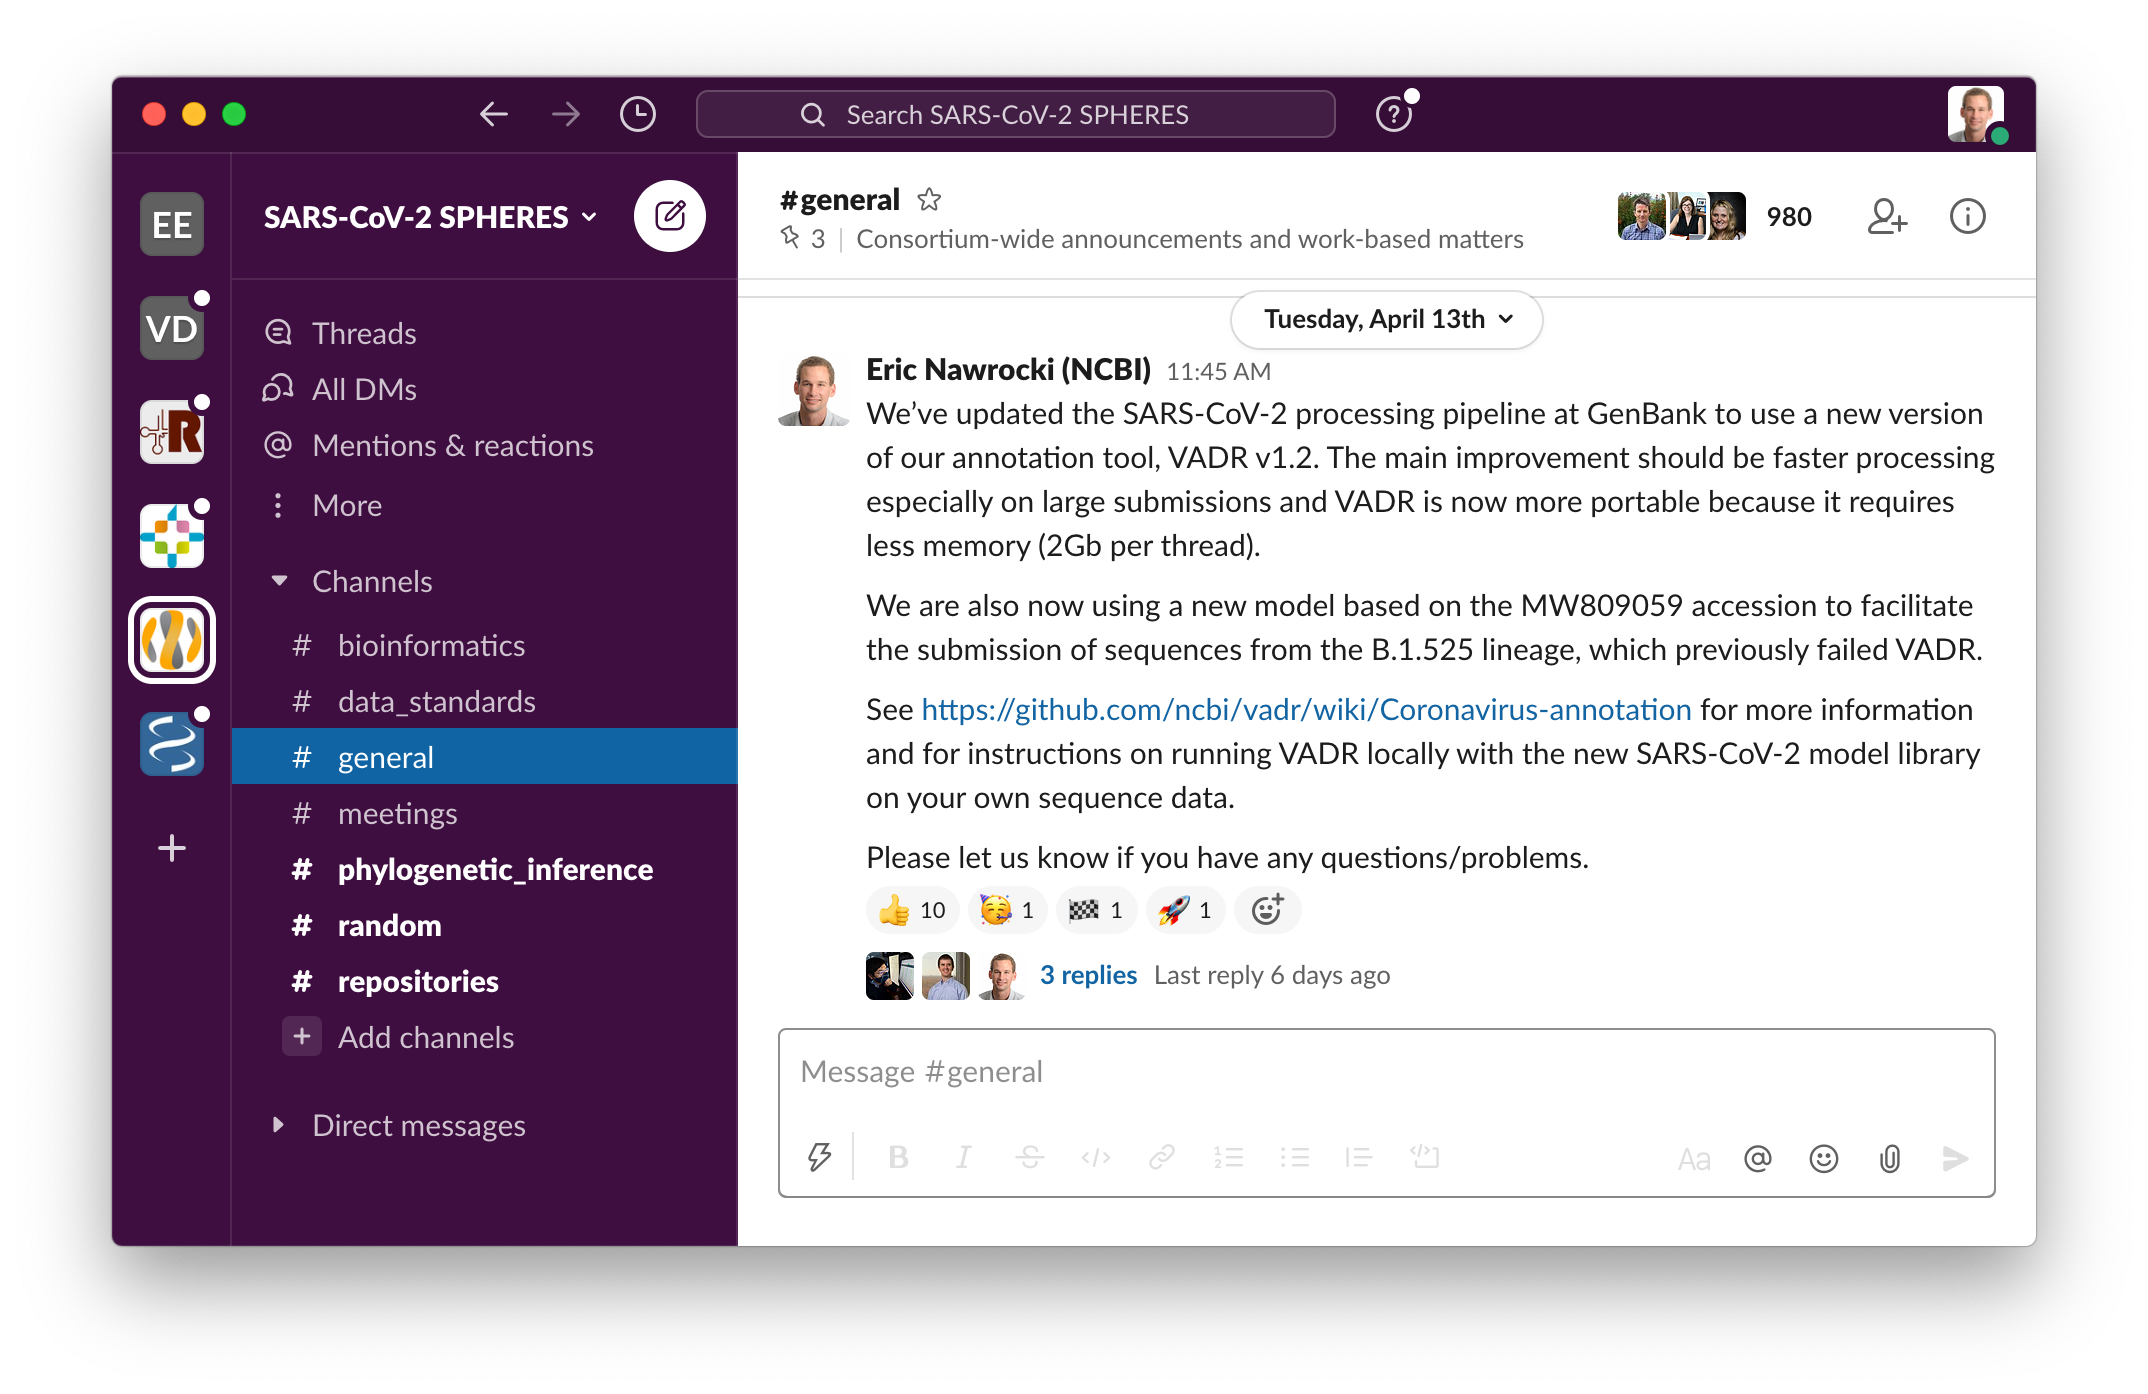
\includegraphics[width=8.5in]{figs/spheres-slack-apr132021}

\small
\begin{itemize}
\item VADR is portable and is run locally by labs on their sequences prior to submission
%\item Docker container (thanks to Curtis Kapsak and StaPH-B) adds to portability
\item SPHERES/CDC alert us of problems with VADR and model coverage
%\item We have weekly calls with CDC and receive questions and feature requests
\end{itemize}

\end{center}

\vfill
\end{slide}
%%%%%%%%%%%%%%%%%%%%%%%%%%%%%%%%%%%%%%%%%%%%%%%%%%%%%%%%%%%%%%%%%%%%%%
%\begin{slide}
%\begin{center}
%\large{\textbf{We actively support (and are supported by) the SPHERES community}}
%
%\small
%\begin{itemize}
%\item VADR is portable and is run locally by labs prior to submission
%\item Docker container thanks to Curtis Kapsak and StaPH-B
%\item SPHERES members alert us of problems with VADR and model coverage
%\item We have weekly calls with CDC and receive questions and feature requests
%\end{itemize}
%
%\end{center}
%
%\vfill
%\end{slide}
%%%%%%%%%%%%%%%%%%%%%%%%%%%%%%%%%%%%%%%%%%%%%%%%%%%%%%%%%%%%%%%%%%%%%%
\begin{slide}
\begin{center}
\large{\textbf{Future improvements: VADR 1.2.1 TODO list}}

\normalsize
\begin{itemize}
\item Review list of seqs that fail VADR but should pass
  \begin{itemize}
    \item make changes to code and/or models to accommodate them, if possible
  \end{itemize}
\item Review VADR error messages, and add parseable position data (SPHERES)
\item Update handling of non NNN start/stop codons that translate to X (CDC)
\end{itemize}

\end{center}

\vfill
\end{slide}
%%%%%%%%%%%%%%%%%%%%%%%%%%%%%%%%%%%%%%%%%%%%%%%%%%%%%%%%%%%%%%%%%%%%%%
\begin{slide}

\large
\begin{center}
\large{\textbf{Acknowledgements}} \\

\normalsize
\vspace{0.75in}

\small
\begin{tabular}{l|l|l}
%                  & \\ \hline
%                  & \\
\textbf{NCBI - viral annotation} & \textbf{NCBI - leadership} &  \textbf{Software developers} \\
Alejandro Sch\"{a}ffer (now NCI) & David Landsman             & Sean Eddy (HMMER/Infernal/Easel)\\
                                 & Kim Pruitt                 & Travis Wheeler (HMMER)\\
Ilene Mizrachi                   & Steve Sherry               & Tom Madden and BLAST team \\
Colleen Bollin                   & Jim Ostell                 & William Pearson (FASTA/glsearch) \\
Linda Yankie                     & David Lipman               & Michael Farrar (HMMER/glsearch) \\
Vincent Calhoun                  &                            & \\
Susan Schafer                    & \textbf{NLM - leadership}  & \\
Beverly Underwood                & Patti Brennan              & \\
Vasuki Gobu                      & Jerry Sheehan              & \\
Sergiy Gotvyanskyy               & Valerie Florance           & \\
Alex Kotliarov                   & & \\
& & \\
Rodney Brister                   & & \\
Eneida Hatcher                   & & \\
& & \\
Lara Shonkwiler                  & & \\
Sophia Hu                        & & \\
& & \\
Wratko Hlavina                   & & \\
Eyal Mozes                       & & \\
Ron Patterson                    & & \\
Sumit Saluja                     & & \\ 
\end{tabular}


\includegraphics[width=2.5in]{figs/NIH_NLM_ABRV_2C_4-white}

\includegraphics[width=2.5in]{figs/ncbi-logo}

\end{center}

\vfill
\end{slide}
%%%%%%%%%%%%%%%%%%%%%%%%%%%%%%%%%%%%%%%%%%%%%%%%%%%%%%%%%%%%%%%%%%%%%%
\end{document}
